\documentclass[11pt]{article}

\usepackage{lmodern}
\usepackage[T1]{fontenc}
\usepackage[margin=1in]{geometry}
\usepackage{amsmath,amssymb,amsthm,mathtools}
\usepackage{pgfplots}
\pgfplotsset{compat=1.17}
\usetikzlibrary{arrows.meta,positioning}
\usepackage[colorlinks,linkcolor=blue!60!black,citecolor=green!40!black,urlcolor=blue!60!black]{hyperref}

\emergencystretch=3em

\usepackage{xcolor}

% Two hand-kept data files, whose headers say how each number was computed:
%   q12data.tex     the q = 12 Lean proof and the window of the main theorem;
%   lengthdata.tex  the best window at each length q = 9..12.
% Resolve whether pdflatex runs in paper/ or at the repo root.
\IfFileExists{q12data.tex}{% q12data.tex -- numbers of the q = 12 Lean proof and of the window of the main
% theorem (hand-kept; not generated).
%
% Proof of record: model m12w2, window src/lbcert/q12win/work/final2_q12.json,
% refit src/lbcert/q12win/work/refit96_q12_pm_g18i16.json, 3,789,405 leaves;
% source and logs in the q12 archive of proofs/archives.tsv (Q12/Simple.lean, the
% N0simple theorems, added 2026-10-26).  Checker logs of record: q12/logs/ver
% (verify.txt, nanoda.log, preplay.log; export of Q12.Simple with five theorems,
% 1,750,125,618 bytes).  Verified by both checkers 2026-10-27.  The logs of the
% export with only the three template theorems (2026-10-26) are in
% q12/logs/ver_three_theorems.
%
% How the derived values were computed (2026-10-26):
%   \qKappa...\qB, \qGainMT, \qHbelowMT, \qEnergyMT, \qCeilGap, \qdFdH, \qdFdc,
%   \qDiff...: exact rationals from the Lean source (HW_ge, W13_B, cert_AM),
%     with H_MT and the ceiling 0.681 defined below;
%   \qHmargin: pipeline/hfloor.py H_interval at 60 digits on the window,
%     lower endpoint minus H_W^-;
%   \qVmin, \qVminAt, \qAbsTail, \qPosBound: the minimum of v on [0, 1/2] by a scan
%     of 20,001 points refined six times around the smallest, and the tail sum of the numerators (4379/5760 - 81695290/10^9 = 0.67854...);
%   \qSep...: src/sep_conditions_cert.py --cert
%     src/lbcert/q12win/work/final2_q12_sepinput.json, record
%     results/sep_conditions_final2_q12.json (Arb, 20,000 segments);
%   \qWindowRows: the numerators of final2_q12.json.

% Shared constants.
\newcommand{\qQ}{12}
\newcommand{\qNpts}{13}
\newcommand{\qNpairs}{78}
\newcommand{\qRoots}{9}
\newcommand{\qScale}{2^{23}\cdot10^{24}}
\newcommand{\qRecordNum}{1669044344675499575055516274525441801367}
\newcommand{\qRecordDen}{2477793188117925391575000000000000000000}
\newcommand{\qRecord}{0.6736011514}
\newcommand{\qNineKappa}{0.6736387063}

% The proof of record and its window.
\newcommand{\qWindowFile}{\texttt{final2\_q12.json}}
\newcommand{\qKappaNum}{854046308300026565326564954594528531931648}
\newcommand{\qKappaDen}{1267673952595351605232565361802825927734375}
\newcommand{\qKappa}{0.67371133291}
\newcommand{\qKappaShort}{0.6737113}
\newcommand{\qHnum}{6720761997177286221959388707769754155716}
\newcommand{\qH}{0.6720761997177286}
\newcommand{\qHshort}{0.6720762}
\newcommand{\qHmargin}{7.7\times10^{-41}}
\newcommand{\qcNum}{80779984271103719947859644889}
\newcommand{\qc}{0.0096297245}
\newcommand{\qcShort}{0.0096297}
\newcommand{\qBNum}{40705899486681963457654292480}
\newcommand{\qB}{0.0048525213}
\newcommand{\qDiffNine}{7.26\times10^{-5}}
\newcommand{\qGainMT}{1.21\times10^{-3}}
\newcommand{\qHbelowMT}{4.25\times10^{-4}}
\newcommand{\qEnergyMT}{1.64\times10^{-3}}
\newcommand{\qCeilGap}{7.3\times10^{-3}}
\newcommand{\qdFdH}{1.010}
\newcommand{\qdFdc}{0.680}
\newcommand{\qAbsTail}{81\,695\,290}
\newcommand{\qPosBound}{0.678}
\newcommand{\qVmin}{0.7357}
\newcommand{\qVminAt}{0.466}
\newcommand{\qSepMajMargin}{0.1322}
\newcommand{\qSepLam}{1.9271}
\newcommand{\qSepCloseMargin}{0.1012}
\newcommand{\qWindowRows}{%
$0$ & $\sqrt2$ & $1\,000\,000\,000$ & $6$ & $12\pi$ & $2\,247\,687$ & $12$ & $24\pi$ & $3\,521\,384$\\
$1$ & $2\pi$ & $14\,564\,693$ & $7$ & $14\pi$ & $-4\,183\,770$ & $13$ & $26\pi$ & $-3\,153\,149$\\
$2$ & $4\pi$ & $-17\,645\,853$ & $8$ & $16\pi$ & $1\,416\,728$ & $14$ & $28\pi$ & $3\,602\,408$\\
$3$ & $6\pi$ & $7\,869\,625$ & $9$ & $18\pi$ & $-3\,647\,215$ & $15$ & $30\pi$ & $-3\,727\,658$\\
$4$ & $8\pi$ & $4\,852\,247$ & $10$ & $20\pi$ & $4\,135\,017$ & $16$ & $32\pi$ & $3\,294\,246$\\
$5$ & $10\pi$ & $1\,453\,496$ & $11$ & $22\pi$ & $-2\,380\,114$ &  &  & \\}
\newcommand{\qLeaves}{3\,789\,405}
\newcommand{\qRefl}{566\,603}
\newcommand{\qModules}{143}
\newcommand{\qCuts}{19\,901}
\newcommand{\qPoints}{31\,073}
\newcommand{\qSource}{425.3\,MB}
\newcommand{\qExport}{1.75\,GB}
\newcommand{\qConstants}{332\,379}
\newcommand{\qNanodaTime}{6.10\,h}
\newcommand{\qNanodaMem}{14.4\,GB}
\newcommand{\qReplayTime}{3.88\,h}
\newcommand{\qReplayMem}{15.0\,GB}
\newcommand{\qVerifiedDate}{October 27, 2026}

% Window family and constants that do not depend on the certificate.
% H_MT = 3/2 - cot(1/sqrt 2)/sqrt 2; the ceiling is the numerical estimate of
% Section sec:limits; gamma_Delta and the
% segment count are those of results/sep_conditions_final2_q12.json.
\newcommand{\qNharm}{16}
\newcommand{\qNharmWordCap}{Sixteen}
\newcommand{\qCden}{10^{9}}
\newcommand{\qHMT}{0.6725007}
\newcommand{\qHMTlong}{0.6725007036794116}
\newcommand{\qCeiling}{0.681}
\newcommand{\qSepGamma}{7/10}
\newcommand{\qSepSegments}{20\,000}
}{% q12data.tex -- numbers of the q = 12 Lean proof and of the window of the main
% theorem (hand-kept; not generated).
%
% Proof of record: model m12w2, window src/lbcert/q12win/work/final2_q12.json,
% refit src/lbcert/q12win/work/refit96_q12_pm_g18i16.json, 3,789,405 leaves;
% source and logs in the q12 archive of proofs/archives.tsv (Q12/Simple.lean, the
% N0simple theorems, added 2026-10-26).  Checker logs of record: q12/logs/ver
% (verify.txt, nanoda.log, preplay.log; export of Q12.Simple with five theorems,
% 1,750,125,618 bytes).  Verified by both checkers 2026-10-27.  The logs of the
% export with only the three template theorems (2026-10-26) are in
% q12/logs/ver_three_theorems.
%
% How the derived values were computed (2026-10-26):
%   \qKappa...\qB, \qGainMT, \qHbelowMT, \qEnergyMT, \qCeilGap, \qdFdH, \qdFdc,
%   \qDiff...: exact rationals from the Lean source (HW_ge, W13_B, cert_AM),
%     with H_MT and the ceiling 0.681 defined below;
%   \qHmargin: pipeline/hfloor.py H_interval at 60 digits on the window,
%     lower endpoint minus H_W^-;
%   \qVmin, \qVminAt, \qAbsTail, \qPosBound: the minimum of v on [0, 1/2] by a scan
%     of 20,001 points refined six times around the smallest, and the tail sum of the numerators (4379/5760 - 81695290/10^9 = 0.67854...);
%   \qSep...: src/sep_conditions_cert.py --cert
%     src/lbcert/q12win/work/final2_q12_sepinput.json, record
%     results/sep_conditions_final2_q12.json (Arb, 20,000 segments);
%   \qWindowRows: the numerators of final2_q12.json.

% Shared constants.
\newcommand{\qQ}{12}
\newcommand{\qNpts}{13}
\newcommand{\qNpairs}{78}
\newcommand{\qRoots}{9}
\newcommand{\qScale}{2^{23}\cdot10^{24}}
\newcommand{\qRecordNum}{1669044344675499575055516274525441801367}
\newcommand{\qRecordDen}{2477793188117925391575000000000000000000}
\newcommand{\qRecord}{0.6736011514}
\newcommand{\qNineKappa}{0.6736387063}

% The proof of record and its window.
\newcommand{\qWindowFile}{\texttt{final2\_q12.json}}
\newcommand{\qKappaNum}{854046308300026565326564954594528531931648}
\newcommand{\qKappaDen}{1267673952595351605232565361802825927734375}
\newcommand{\qKappa}{0.67371133291}
\newcommand{\qKappaShort}{0.6737113}
\newcommand{\qHnum}{6720761997177286221959388707769754155716}
\newcommand{\qH}{0.6720761997177286}
\newcommand{\qHshort}{0.6720762}
\newcommand{\qHmargin}{7.7\times10^{-41}}
\newcommand{\qcNum}{80779984271103719947859644889}
\newcommand{\qc}{0.0096297245}
\newcommand{\qcShort}{0.0096297}
\newcommand{\qBNum}{40705899486681963457654292480}
\newcommand{\qB}{0.0048525213}
\newcommand{\qDiffNine}{7.26\times10^{-5}}
\newcommand{\qGainMT}{1.21\times10^{-3}}
\newcommand{\qHbelowMT}{4.25\times10^{-4}}
\newcommand{\qEnergyMT}{1.64\times10^{-3}}
\newcommand{\qCeilGap}{7.3\times10^{-3}}
\newcommand{\qdFdH}{1.010}
\newcommand{\qdFdc}{0.680}
\newcommand{\qAbsTail}{81\,695\,290}
\newcommand{\qPosBound}{0.678}
\newcommand{\qVmin}{0.7357}
\newcommand{\qVminAt}{0.466}
\newcommand{\qSepMajMargin}{0.1322}
\newcommand{\qSepLam}{1.9271}
\newcommand{\qSepCloseMargin}{0.1012}
\newcommand{\qWindowRows}{%
$0$ & $\sqrt2$ & $1\,000\,000\,000$ & $6$ & $12\pi$ & $2\,247\,687$ & $12$ & $24\pi$ & $3\,521\,384$\\
$1$ & $2\pi$ & $14\,564\,693$ & $7$ & $14\pi$ & $-4\,183\,770$ & $13$ & $26\pi$ & $-3\,153\,149$\\
$2$ & $4\pi$ & $-17\,645\,853$ & $8$ & $16\pi$ & $1\,416\,728$ & $14$ & $28\pi$ & $3\,602\,408$\\
$3$ & $6\pi$ & $7\,869\,625$ & $9$ & $18\pi$ & $-3\,647\,215$ & $15$ & $30\pi$ & $-3\,727\,658$\\
$4$ & $8\pi$ & $4\,852\,247$ & $10$ & $20\pi$ & $4\,135\,017$ & $16$ & $32\pi$ & $3\,294\,246$\\
$5$ & $10\pi$ & $1\,453\,496$ & $11$ & $22\pi$ & $-2\,380\,114$ &  &  & \\}
\newcommand{\qLeaves}{3\,789\,405}
\newcommand{\qRefl}{566\,603}
\newcommand{\qModules}{143}
\newcommand{\qCuts}{19\,901}
\newcommand{\qPoints}{31\,073}
\newcommand{\qSource}{425.3\,MB}
\newcommand{\qExport}{1.75\,GB}
\newcommand{\qConstants}{332\,379}
\newcommand{\qNanodaTime}{6.10\,h}
\newcommand{\qNanodaMem}{14.4\,GB}
\newcommand{\qReplayTime}{3.88\,h}
\newcommand{\qReplayMem}{15.0\,GB}
\newcommand{\qVerifiedDate}{October 27, 2026}

% Window family and constants that do not depend on the certificate.
% H_MT = 3/2 - cot(1/sqrt 2)/sqrt 2; the ceiling is the numerical estimate of
% Section sec:limits; gamma_Delta and the
% segment count are those of results/sep_conditions_final2_q12.json.
\newcommand{\qNharm}{16}
\newcommand{\qNharmWordCap}{Sixteen}
\newcommand{\qCden}{10^{9}}
\newcommand{\qHMT}{0.6725007}
\newcommand{\qHMTlong}{0.6725007036794116}
\newcommand{\qCeiling}{0.681}
\newcommand{\qSepGamma}{7/10}
\newcommand{\qSepSegments}{20\,000}
}
\IfFileExists{lengthdata.tex}{% lengthdata.tex -- the best window at each geometry length q = 9..12
% (Table tab:ladder, Appendix app:ladder; hand-kept, not generated).
%
% Every kappa_L is the exact (H_W^- - B)/(1 - c), c = eps - 6e-7.
% q = 9: the challenge entry rishikhan-ten-point-certificate, window
%   results/sepsearch/best_q9_j16.json, model q9a, cover range K_B = 2^20;
%   kappa from proofs/archives.tsv (row q9); leaves of the submitted file
%   Solution_Zskip.lean in the q9 archive (27,554 + 49 refl).
% q = 10, q = 11: src/lbcert/q12win/work/final_q10.json, final_q11.json (lean_kappa,
%   refit, side_conditions); trees and logs in the q10 and q11 archives.
% q = 12: q12data.tex.
% Steps: exact differences of the kappa_L fractions.  Growth: ratios of tree leaves, refl excluded.
%
% q = 10, q = 11 Lean proofs (2026-10-27): the q10 and q11 archives of proofs/archives.tsv.

% Table rows' entries.
\newcommand{\lenNineKappa}{0.6736387063}
\newcommand{\lenTenKappa}{0.6736701854}
\newcommand{\lenElevenKappa}{0.6736952870}
\newcommand{\lenTwelveKappa}{0.6737113329}
\newcommand{\lenNineFloat}{0.6736391143}
\newcommand{\lenTenFloat}{0.6736705935}
\newcommand{\lenElevenFloat}{0.6736956953}
\newcommand{\lenTwelveFloat}{0.6737117411}
\newcommand{\lenNineB}{0.0047386}
\newcommand{\lenTenB}{0.0047584}
\newcommand{\lenElevenB}{0.0049252}
\newcommand{\lenTwelveB}{0.0048525}
\newcommand{\lenNineLeaves}{27\,554}
\newcommand{\lenNineRefl}{49}
\newcommand{\lenTenLeaves}{221\,123}
\newcommand{\lenTenRefl}{164}
\newcommand{\lenElevenLeaves}{879\,952}
\newcommand{\lenElevenRefl}{380}
\newcommand{\lenNineBytes}{1\,890\,088}
\newcommand{\lenNineVer}{Lean, hosted checker}
\newcommand{\lenTenVer}{Lean, kernel and nanoda}
\newcommand{\lenElevenVer}{Lean, kernel and nanoda}
\newcommand{\lenTwelveVer}{Lean, Theorem~\ref{thm:formal}}

% Steps in kappa_L and leaf growth between lengths.
\newcommand{\lenStepNineTen}{3.15\times10^{-5}}
\newcommand{\lenStepTenEleven}{2.51\times10^{-5}}
\newcommand{\lenStepElevenTwelve}{1.60\times10^{-5}}
\newcommand{\lenGrowthNineTen}{8.0}
\newcommand{\lenGrowthTenEleven}{4.0}
\newcommand{\lenGrowthElevenTwelve}{4.3}

% How the rows are verified (prose of Appendix app:ladder).
\newcommand{\lenVerNote}{The $q=9$ and $q=12$ rows are the Lean proofs of
Section~\ref{sec:q12lean}. The $q=10$ and $q=11$ rows are Lean proofs built by
the same generator as the $q=12$ proof, with the same five exported theorems.
Before generation, two exact rational checks accept every leaf of their trees:
the generator's check in C++, run on the assembled trees and again against the
final table of tangent points, and an independent check in Python, whose leaf
counts and minimum margins equal those of the C++ check in every root box.
The Lean kernel, through a replay of the export ($86\,937$ declarations at
$q=10$, $126\,752$ at $q=11$), and nanoda accept both proofs, and their
theorems depend only on \texttt{propext}, \texttt{Classical.choice} and
\texttt{Quot.sound}. The Arb check of Proposition~\ref{prop:inputs} gives (W1)
and (W2) for these two windows with margins at least $0.127$ and $0.101$.}
}{% lengthdata.tex -- the best window at each geometry length q = 9..12
% (Table tab:ladder, Appendix app:ladder; hand-kept, not generated).
%
% Every kappa_L is the exact (H_W^- - B)/(1 - c), c = eps - 6e-7.
% q = 9: the challenge entry rishikhan-ten-point-certificate, window
%   results/sepsearch/best_q9_j16.json, model q9a, cover range K_B = 2^20;
%   kappa from proofs/archives.tsv (row q9); leaves of the submitted file
%   Solution_Zskip.lean in the q9 archive (27,554 + 49 refl).
% q = 10, q = 11: src/lbcert/q12win/work/final_q10.json, final_q11.json (lean_kappa,
%   refit, side_conditions); trees and logs in the q10 and q11 archives.
% q = 12: q12data.tex.
% Steps: exact differences of the kappa_L fractions.  Growth: ratios of tree leaves, refl excluded.
%
% q = 10, q = 11 Lean proofs (2026-10-27): the q10 and q11 archives of proofs/archives.tsv.

% Table rows' entries.
\newcommand{\lenNineKappa}{0.6736387063}
\newcommand{\lenTenKappa}{0.6736701854}
\newcommand{\lenElevenKappa}{0.6736952870}
\newcommand{\lenTwelveKappa}{0.6737113329}
\newcommand{\lenNineFloat}{0.6736391143}
\newcommand{\lenTenFloat}{0.6736705935}
\newcommand{\lenElevenFloat}{0.6736956953}
\newcommand{\lenTwelveFloat}{0.6737117411}
\newcommand{\lenNineB}{0.0047386}
\newcommand{\lenTenB}{0.0047584}
\newcommand{\lenElevenB}{0.0049252}
\newcommand{\lenTwelveB}{0.0048525}
\newcommand{\lenNineLeaves}{27\,554}
\newcommand{\lenNineRefl}{49}
\newcommand{\lenTenLeaves}{221\,123}
\newcommand{\lenTenRefl}{164}
\newcommand{\lenElevenLeaves}{879\,952}
\newcommand{\lenElevenRefl}{380}
\newcommand{\lenNineBytes}{1\,890\,088}
\newcommand{\lenNineVer}{Lean, hosted checker}
\newcommand{\lenTenVer}{Lean, kernel and nanoda}
\newcommand{\lenElevenVer}{Lean, kernel and nanoda}
\newcommand{\lenTwelveVer}{Lean, Theorem~\ref{thm:formal}}

% Steps in kappa_L and leaf growth between lengths.
\newcommand{\lenStepNineTen}{3.15\times10^{-5}}
\newcommand{\lenStepTenEleven}{2.51\times10^{-5}}
\newcommand{\lenStepElevenTwelve}{1.60\times10^{-5}}
\newcommand{\lenGrowthNineTen}{8.0}
\newcommand{\lenGrowthTenEleven}{4.0}
\newcommand{\lenGrowthElevenTwelve}{4.3}

% How the rows are verified (prose of Appendix app:ladder).
\newcommand{\lenVerNote}{The $q=9$ and $q=12$ rows are the Lean proofs of
Section~\ref{sec:q12lean}. The $q=10$ and $q=11$ rows are Lean proofs built by
the same generator as the $q=12$ proof, with the same five exported theorems.
Before generation, two exact rational checks accept every leaf of their trees:
the generator's check in C++, run on the assembled trees and again against the
final table of tangent points, and an independent check in Python, whose leaf
counts and minimum margins equal those of the C++ check in every root box.
The Lean kernel, through a replay of the export ($86\,937$ declarations at
$q=10$, $126\,752$ at $q=11$), and nanoda accept both proofs, and their
theorems depend only on \texttt{propext}, \texttt{Classical.choice} and
\texttt{Quot.sound}. The Arb check of Proposition~\ref{prop:inputs} gives (W1)
and (W2) for these two windows with margins at least $0.127$ and $0.101$.}
}

% A visible marker for a statement the authors have to confirm.
\newcommand{\todo}[1]{\textcolor{red}{[TODO: #1]}}

\newtheorem{theorem}{Theorem}[section]
\newtheorem{proposition}[theorem]{Proposition}
\newtheorem{lemma}[theorem]{Lemma}
\newtheorem{corollary}[theorem]{Corollary}
\theoremstyle{definition}
\newtheorem{remark}[theorem]{Remark}

\DeclareMathOperator{\tr}{tr}
\DeclareMathOperator{\rank}{rank}
\newcommand{\R}{\mathbb{R}}
\newcommand{\Z}{\mathbb{Z}}
\newcommand{\F}{\mathrm{F}}
\newcommand{\Fr}{\mathcal{F}}
\newcommand{\cS}{\mathcal{S}}
\newcommand{\cP}{\mathcal{P}}
\newcommand{\cR}{\mathcal{R}}
\newcommand{\eps}{\varepsilon}

\title{A formally verified lower bound of \\ $\qKappaShort$ for the proportion of simple critical-line zeros \\ of the Riemann zeta function}
\author{Rishi Khan \and Albert DeWeese}
\date{October 27, 2026}

\begin{document}
\maketitle

\begin{abstract}
Let $N(T,2T)$ count the nontrivial zeros of the Riemann zeta function with
ordinates in $(T,2T]$, with multiplicity, and let $N_0^s(T,2T)$ count the
zeros in that interval that are simple and lie on the critical line. We prove
unconditionally that
\[
  \liminf_{T\to\infty}\frac{N_0^s(T,2T)}{N(T,2T)}\;\ge\;\kappa_L,
\]
where
\[
  \kappa_L:=\frac{\qKappaNum}{\qKappaDen}=\qKappa\ldots .
\]
Let $N_0^*(T,2T)$ count the distinct zeros on the critical line with
ordinates in $(T,2T]$. The constant has the form $\kappa_L=(H_W^--B)/(1-c)$: $H_W^-$ is a rational floor of the
window form factor $H=2-W(v)$ given by Montgomery's unconditional
pair-correlation theorem, $B$ is a pressure, and $c$ is a forced local energy
that a $\qNpts$-point local functional certifies over all nonnegative gaps. A
proof written in Lean~4 against Mathlib, built on the Lean formalization of
the reduction of Alp\"oge and Furman~\cite{Zeta23Lean} and on the Lean proofs
of the \texttt{riemannzeta.fun} challenge~\cite{RZF26,Lav26}, proves
$(\kappa_L-\eps)N(T,2T)\le N_0^s(T,2T)$ for every $\eps>0$ and all large $T$,
which gives the bound above, and the same on the intervals $(0,T]$; it also
states both inequalities for $N_0^*$. The Lean kernel, through a replay of
the exported proof, and the independent checker nanoda both accept all
declarations, and the theorems depend only on the axioms \texttt{propext},
\texttt{Classical.choice} and \texttt{Quot.sound}. The kernel evaluates the
certificate of $c$ as a tree of boxes with $\qLeaves$ leaves. We also prove
the bound in writing, from Weil's explicit formula, the unconditional
Montgomery moments and finite-dimensional linear algebra, with the
Lean-checked certificate of $c$ as its computed input. The bound improves
$H_{\mathrm{MT}}=\qHMT$~\cite{AF26}. Numerical optimization
over the window families examined here places the ceiling of the method, the
pair-correlation second moment on bandwidth $|\alpha|\le1$, near
$\qCeiling$. The bound is a limit inferior and carries no explicit
finite~$T$.
\end{abstract}

\section{Introduction}\label{sec:intro}

\subsection{Problem and prior bounds}
Write $\rho=\beta+i\gamma$ for a nontrivial zero of $\zeta(s)$ with
multiplicity $m_\rho\ge1$, and for $0\le T_1<T_2$ set
\[
  N(T_1,T_2):=\sum_{T_1<\gamma\le T_2}m_\rho,\qquad
  N_0^s(T_1,T_2):=\#\{\rho:\,T_1<\gamma\le T_2,\ \beta=\tfrac12,\ m_\rho=1\},
\]
and let $N_0^*(T_1,T_2)$ count the distinct zeros with $T_1<\gamma\le T_2$
and $\beta=\tfrac12$, each once whatever its multiplicity, so
$N_0^s\le N_0^*$.
Call a zero \emph{on-line} when $\beta=\tfrac12$ and \emph{off-line}
otherwise. The quantity $N_0^s/N$ measures the proportion of the zeta zeros
that are simultaneously simple and on-line. Pratt, Robles, Zaharescu, and Zeindler~\cite{PRZZ20} prove that more than
$5/12$ of the zeros lie on the critical line, and report $\kappa>0.417293$ on
an interim optimization of their parameters, together with
$\kappa^{*}\ge0.407511$ for the proportion that is also simple, the transfer
between the two being Heath-Brown's~\cite{HB79}. So $5/12$ is the on-line
figure, and $\kappa^{*}$ is the earlier bound for the proportion of interest
here. Alp\"oge and Furman~\cite{AF26} raised it to
\[
  H_{\mathrm{MT}}:=\tfrac32-\tfrac1{\sqrt2}\cot\tfrac1{\sqrt2}
  =\qHMTlong\ldots,
\]
attained with the Montgomery--Taylor window, and proved this optimal within its
window family. Their argument is formalized in Lean~4~\cite{Zeta23Lean}, and
the \texttt{riemannzeta.fun} challenge~\cite{RZF26} accepts Lean proofs of
larger constants built on that formalization. Its leading entries in October
2026 prove bounds of the form $(H_W^--B)/(1-c)$ for $N_0^s$ and state them for
$N_0^*$; the largest before October 25, 2026 was $\qRecord$.
% Leaderboard state taken from the project notes of 2026-10-25; check
% data/records.json of the challenge repository before publication.
Our entry at
$q=9$, which uses the method of Section~\ref{sec:q12lean} with a ten-point
certificate, was accepted on October 25, 2026 with $\kappa=\qNineKappa$.

The main result is the following theorem.

\begin{theorem}[Main theorem]\label{thm:main}
Let
\[
  \kappa_L:=\frac{\qKappaNum}{\qKappaDen}=\qKappa\ldots .
\]
Then
\begin{equation}\label{eq:main-number}
  \liminf_{T\to\infty}\frac{N_0^s(T,2T)}{N(T,2T)}\ge\kappa_L .
\end{equation}
\end{theorem}

Theorem~\ref{thm:main} follows from the dyadic inequality for $N_0^s$ of
Theorem~\ref{thm:formal}: dividing by $N(T,2T)>0$ gives a limit inferior of at
least $\kappa_L-\eps$ for every $\eps>0$. The Lean kernel and nanoda check that
inequality as the theorem \texttt{candidate\_simple\_critical\_line\_bound},
whose proof starts from Mathlib's definition of $\zeta$ and takes no
hypothesis (Section~\ref{sec:q12lean}). Section~\ref{sec:main} also proves
Theorem~\ref{thm:main} by the written argument of
Sections~\ref{sec:framework}--\ref{sec:separated}, with three computed inputs
for the window of Table~\ref{tab:window}: the forced local energy $c$ of
Section~\ref{sec:cert}, which the Lean kernel checks
(Section~\ref{sec:q12lean}), and the $H$ floor and the window conditions,
which are computed in Arb ball arithmetic and also proved in Lean.

\begin{theorem}[Formally verified bound]\label{thm:formal}
For every $\eps>0$ there is $T_0$ such that for all $T\ge T_0$
\[
  (\kappa_L-\eps)\,N(T,2T)\le N_0^s(T,2T),\qquad
  (\kappa_L-\eps)\,N(0,T)\le N_0^s(0,T),
\]
and the same two inequalities hold with $N_0^*$ in place of $N_0^s$.
\end{theorem}

The bounds for $N_0^*$ follow from those for $N_0^s$, since
$N_0^s\le N_0^*$; the Lean proof states them because the challenge's
candidate template~\cite{RZF26} states $N_0^*$.
Conditional results under the Riemann
hypothesis are numerically stronger. They furnish no unconditional lower
bound, so they do not bear on~\eqref{eq:main-number}.

\subsection{Method}
Reading Weil's explicit formula as a Hermitian form and evaluating Montgomery's
first and second moments gives the defect inequality
$N_0^s/N\ge H+\mathcal D(M^\circ)/N-o(1)$, where $H:=2-W(v)$ is a window form
factor and $\mathcal D(M^\circ)\ge0$ is the spectral defect of the Gram matrix of
the simple critical-line zeros. Dropping the defect gives $N_0^s/N\ge H$, and the
Montgomery--Taylor window makes $H=H_{\mathrm{MT}}$.
Section~\ref{sec:framework} re-derives this reduction from the explicit formula
(Iwaniec--Kowalski), the unconditional Montgomery moments (Aryan; Baluyot,
Goldston, Suriajaya, and Turnage-Butterbaugh, following Montgomery), and the
linear algebra of Appendix~\ref{app:inertia}. The normalizations carrying
Proposition~\ref{prop:moment} to~\eqref{eq:moments} are assumed rather than
proved, and input~(A5) names them. We prove a strictly positive lower
bound on $\mathcal D(M^\circ)/N$. First, zeros closer than $\Delta=17/20$
of the mean spacing are matched in pairs, and each pair carries defect at
least $1/32$. Second, on the $\Delta$-separated remainder a two-sinc majorant
of the window caps the Gram eigenvalues below $2$, at every height and for
sets of any size, so the defect of the remainder equals its off-diagonal
energy, and the span capacities bound that energy below by the forced local
energy of its windows minus their pressure. Pinching adds the two parts with
no loss. Third, the forced local energy is \emph{certified}: a rigorous lower
bound on the minimum of an explicit local functional over the nonnegative gap
orthant. For the window of Table~\ref{tab:window} the certificate is a tree of
boxes that the Lean kernel evaluates, at $q=\qQ$ with $\qNpts$ points and
pair weights and pressures fitted for the separated assembly
(Section~\ref{sec:q12lean}); it gives Theorem~\ref{thm:main}. Figure~\ref{fig:flow} shows how the
steps compose and marks each as an external input, proved here, or certified
by computation.

The proof of Theorem~\ref{thm:formal} follows the same three steps inside Lean
(Section~\ref{sec:q12lean}). It takes the reduction from the Lean
formalization~\cite{Zeta23Lean} of~\cite{AF26} and the matching, the
eigenvalue cap and the counting from the Lean proofs of the
\texttt{riemannzeta.fun} challenge~\cite{RZF26,Lav26}, so it uses neither
Section~\ref{sec:framework} nor input~(A5).

\begin{figure}[t]
\centering
\resizebox{\textwidth}{!}{%
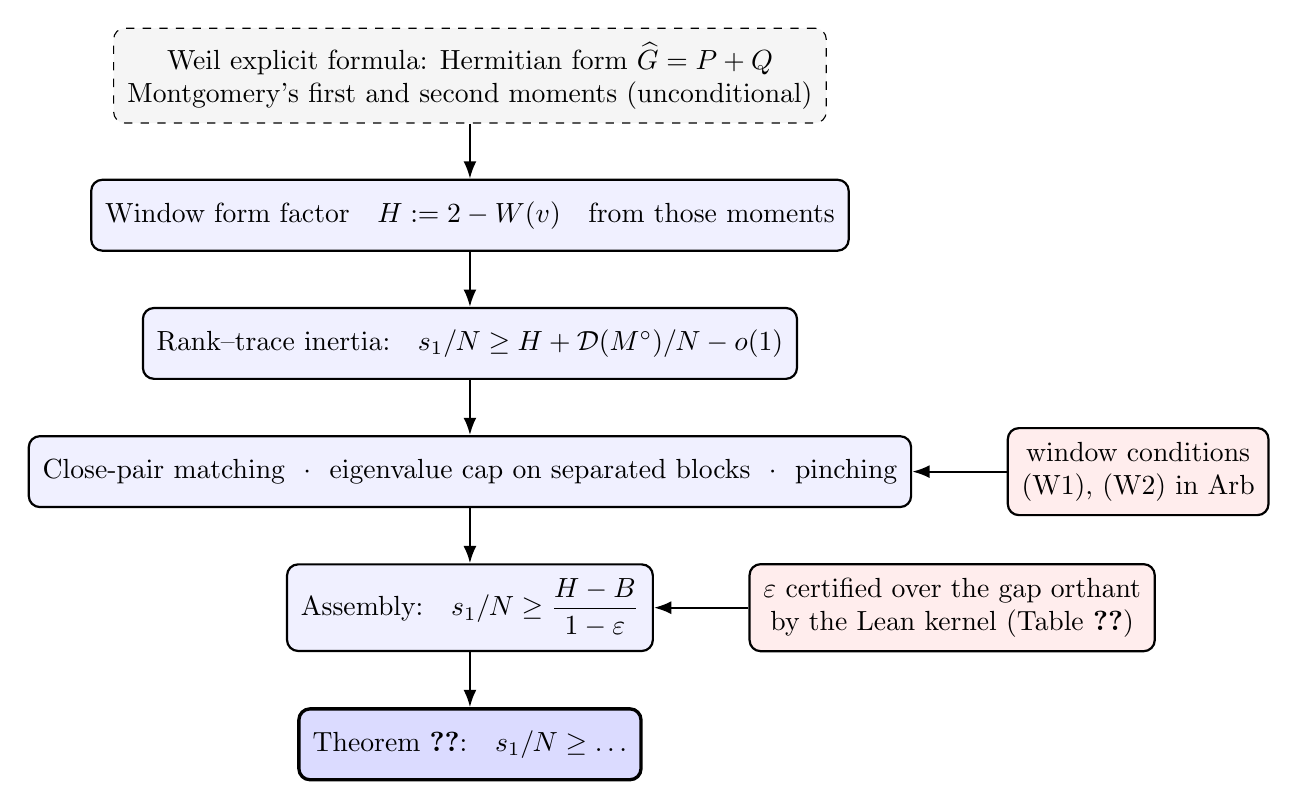
\begin{tikzpicture}[
  node distance=7mm,
  box/.style={draw, rounded corners, align=center, inner sep=5pt,
              minimum height=9mm},
  inh/.style={box, dashed, fill=black!4},
  prv/.style={box, thick, fill=blue!6},
  cmp/.style={box, thick, fill=red!7},
  res/.style={box, very thick, fill=blue!14},
  arr/.style={-{Latex[length=2.2mm]}, thick},
]
\node[inh] (n1) {Weil explicit formula: Hermitian form $\widehat G=P+Q$\\
  Montgomery's first and second moments (unconditional)};
\node[prv, below=of n1] (n2) {Window form factor\quad $H:=2-W(v)$\quad
  from those moments};
\node[prv, below=of n2] (n3) {Rank--trace inertia:\quad
  $s_1/N \ge H + \mathcal D(M^\circ)/N - o(1)$};
\node[prv, below=of n3] (n4) {Close-pair matching \ $\cdot$ \
  eigenvalue cap on separated blocks \ $\cdot$ \ pinching};
\node[prv, below=of n4] (n5) {Assembly:\quad
  $s_1/N \ge \displaystyle\frac{H-B}{1-\eps}$};
\node[res, below=of n5] (n6) {Theorem~\ref{thm:main}:\quad
  $s_1/N \ge \qKappa\ldots$};
\node[cmp, right=12mm of n5] (eps) {$\eps$ certified over the gap orthant\\
  by the Lean kernel (Table~\ref{tab:window})};
\node[cmp, right=12mm of n4] (win) {window conditions\\ (W1), (W2) in Arb};
\draw[arr] (n1)--(n2); \draw[arr] (n2)--(n3); \draw[arr] (n3)--(n4);
\draw[arr] (n4)--(n5); \draw[arr] (n5)--(n6); \draw[arr] (eps)--(n5);
\draw[arr] (win)--(n4);
\end{tikzpicture}}
\caption{Structure of the argument. The dashed box holds the external inputs:
Weil's explicit formula (textbook) and the unconditional Montgomery moments
(refereed). Solid blue boxes are derived or proved here (Section~\ref{sec:framework},
Appendix~\ref{app:inertia}, Section~\ref{sec:separated}); the red boxes are
the inputs certified by computation, the forced local energy $\eps$ and the
window conditions of Section~\ref{sec:separated}. Every other step is
analytic. The formal proof of
Theorem~\ref{thm:formal} follows the same chain with its own inputs
(Section~\ref{sec:q12lean}). Here $s_1$ counts the simple on-line zeros the
argument retains (Appendix~\ref{app:inertia}); input~(A4) gives $s_1\le
N_0^s(T,2T)+o(N)$, which carries the last line to Theorem~\ref{thm:main}. $B$
is the total per-window pressure coefficient of Lemma~\ref{lem:sepdefect},
and $q$ the length of the local functional.}
\label{fig:flow}
\end{figure}

\subsection{Statements proved, cited, and computed}\label{sec:claims}
\begin{itemize}
\item[(i)] \emph{Unconditional analytic theorems proved here:} the eigenvalue
cap on separated blocks (Lemma~\ref{lem:cap}), the close-pair and
separated-defect bounds (Lemmas~\ref{lem:closepair} and~\ref{lem:sepdefect}),
and the separated assembly (Theorem~\ref{thm:sep-assembly}); and the reduction to the
defect inequality~\eqref{eq:global-defect} (Section~\ref{sec:framework}), whose
linear-algebra and counting content is proved in Appendix~\ref{app:inertia}.
\item[(ii)] \emph{Textbook and already-refereed inputs:} Weil's explicit formula
(Iwaniec--Kowalski~\cite[Theorem~5.11]{IK04}); the unconditional Montgomery pair-correlation
theorem (Baluyot, Goldston, Suriajaya, and
Turnage-Butterbaugh~\cite{BGSTB24}, following Montgomery~\cite{Mon73,Mon75}), which
evaluates the second moment and so carries the prime side and the kernel limit;
and the classical tail estimates
(Titchmarsh~\cite{Tit86}; Montgomery--Vaughan~\cite{MV07}) controlling the $o(1)$
errors. These enter Section~\ref{sec:framework} and Appendix~\ref{app:inertia}.
\item[(iii)] \emph{Certified computation:} the forced local energy over the
gap orthant for the window of Table~\ref{tab:window}, as a tree of boxes that
the Lean kernel evaluates (Section~\ref{sec:q12lean}); the $H$ floor and the
window conditions (W1) and (W2), checked in Arb ball arithmetic.
\item[(iv)] \emph{Formally verified, unconditionally:} Theorem~\ref{thm:formal},
for $N_0^s$ and for $N_0^*$, and with it Theorem~\ref{thm:main}. Its Lean
proof starts from Mathlib's definition of $\zeta$ and takes no hypothesis; it
depends on the Lean formalization~\cite{Zeta23Lean} of~\cite{AF26} for the
inputs of (ii), not on Section~\ref{sec:framework}
(Section~\ref{sec:q12lean}). The kernel also checks the $H$ floor, the window
conditions and the certificate for the window of Table~\ref{tab:window} as
declarations.
\end{itemize}

\section{Framework}\label{sec:framework}

This section fixes notation and derives the reduction used in the rest of the paper
from Weil's explicit formula, the unconditional Montgomery
moments, and finite-dimensional linear algebra. The analytic inputs are textbook
or already refereed; the linear-algebra content is proved in
Appendix~\ref{app:inertia}.

\subsection{Weil's explicit formula and the sampling matrix}\label{sec:gabor}
For a zero $\rho$ write $\gamma_\rho:=(\rho-\tfrac12)/i$, the spectral
parameter; it is real and equal to the ordinate $\gamma$ if and only if $\rho$
lies on the critical line, and complex otherwise. Fourier transforms are
normalized by $\widehat f(z):=\int_\R f(u)e^{-izu}\,du$, entire in $z$ when $f$
has compact support, and convolution by
$(f\star h)(u):=\int_\R f(t)h(u-t)\,dt$. For
$f,g\in C^\infty_c(\R)$ with $\operatorname{supp}f,\operatorname{supp}g\subset[-L/2,L/2]$
put $\tilde g(u):=\overline{g(-u)}$; then $\widehat{f\star\tilde g}(z)
=\widehat f(z)\,\overline{\widehat g(\bar z)}$ for every complex $z$. Weil's explicit
formula applied to $f\star\tilde g$ makes
\[
  W(f,g)=\sum_\rho m_\rho\,\widehat f(\gamma_\rho)\,\overline{\widehat g(\overline{\gamma_\rho})}
       =\int_\R \widehat f(\tau)\,\overline{\widehat g(\tau)}\,\nu_X(\tau)\,d\tau
\]
a Hermitian form on this space (no evenness of $f,g$ is required; the
modulated test functions $f_k$ of Section~\ref{sec:gabor} are not even), where
$\nu_X=\mu+\Pi_X+P_X$ collects the archimedean density $\mu$ (from
$\Gamma'/\Gamma$), the pole term $\Pi_X$, and the prime sum
$P_X(\tau)=-\pi^{-1}\sum_{n\le X}\Lambda(n)n^{-1/2}\cos(\tau\log n)$, with $X=e^{L}$.
Proposition~\ref{prop:weil} carries out the passage from the Mellin form of the
explicit formula, Iwaniec--Kowalski~\cite[Theorem~5.11]{IK04}, to this
sesquilinear form. Positivity of $W$ on all of $C^\infty_c(\R)$ is equivalent to
the Riemann hypothesis, but positivity is not used.

\begin{proposition}[Sesquilinear form of the explicit formula]\label{prop:weil}
Let $L>0$, let $f,g\in C^\infty_c(\R)$ have support in $[-L/2,L/2]$, and put
$\tilde g(u)=\overline{g(-u)}$ and $F=f\star\tilde g$.
\begin{enumerate}
\item[(i)] $F\in C^\infty_c(\R)$ with $\operatorname{supp}F\subset[-L,L]$, and
$\widehat F(z)=\widehat f(z)\,\overline{\widehat g(\bar z)}$ for every
$z\in\mathbb{C}$, both sides entire.
\item[(ii)] $\varphi(x):=x^{-1/2}F(\log x)$ is $C^\infty$ on $]0,+\infty[$ with
support in $[e^{-L},e^{L}]$, so it satisfies the hypothesis
of~\cite[Theorem~5.11]{IK04}, and its Mellin transform
$\widehat\varphi(s)=\int_0^{+\infty}\varphi(x)x^{s-1}dx$ is entire with
$\widehat\varphi(\tfrac12+iz)=\widehat F(-z)$ for every $z\in\mathbb{C}$.
\item[(iii)] With $\psi(x)=x^{-1}\varphi(x^{-1})$ and
$\gamma(s)=\pi^{-s/2}\Gamma(s/2)$,
\begin{align*}
  \sum_n\Lambda(n)\big(\varphi(n)+\psi(n)\big)
  &=-\int_\R\widehat F(\tau)\,P_X(\tau)\,d\tau\qquad(X=e^{L}),\\
  \frac{1}{2\pi i}\int_{(1/2)}\Big(\frac{\gamma'}{\gamma}(s)+\frac{\gamma'}{\gamma}(1-s)\Big)\widehat\varphi(s)\,ds
  &=\int_\R\widehat F(\tau)\,\mu(\tau)\,d\tau,
\end{align*}
where $\mu(\tau)=(2\pi)^{-1}\big(\operatorname{Re}\tfrac{\Gamma'}{\Gamma}(\tfrac14+\tfrac{i\tau}{2})-\log\pi\big)$.
The prime sum on the left is finite, running over $n\le e^{L}$ alone.
\item[(iv)] The zero sum
$W(f,g)=\sum_\rho m_\rho\widehat f(\gamma_\rho)\overline{\widehat g(\overline{\gamma_\rho})}$
converges absolutely, and~\cite[Theorem~5.11]{IK04} applied to $\varphi$ gives
\[
  W(f,g)=\Pi_X(f,g)+\int_\R\widehat f(\tau)\,\overline{\widehat g(\tau)}\,
        \big(\mu(\tau)+P_X(\tau)\big)\,d\tau ,
\]
which is the identity of Proposition~\ref{prop:weil} with $\nu_X=\mu+\Pi_X+P_X$. Here
$\Pi_X(f,g)$ is the contribution of the pole of $\zeta$ at $s=1$ together with
the poles of the gamma factors crossed in the contour shift that
proves~\cite[Theorem~5.11]{IK04}; it is a combination of the values
$\widehat F(\pm i/2)$ rather than an integral against a density on $\R$, and the
integral notation in the display absorbs it. It is taken as input; no step of the argument
uses its value.
\item[(v)] $W$ is linear in $f$, conjugate-linear in $g$, and Hermitian:
$W(g,f)=\overline{W(f,g)}$. Hence $\Pi_X$ is Hermitian as well.
\end{enumerate}
\end{proposition}

\begin{proof}
(i) $\tilde g\in C^\infty_c(\R)$ has support in $[-L/2,L/2]$, so $F$ is
$C^\infty$ with support in the sum set $[-L,L]$. Both $\widehat F(z)$ and
$\widehat f(z)\overline{\widehat g(\bar z)}=\widehat f(z)\int_\R\overline{g(u)}e^{-izu}du$
are entire. For real $\tau$,
$\widehat{\tilde g}(\tau)=\int_\R\overline{g(-u)}e^{-i\tau u}du=\overline{\widehat g(\tau)}$
and $\widehat F=\widehat f\,\widehat{\tilde g}$, so the two entire functions agree
on $\R$ and therefore everywhere.

(ii) $\varphi$ is a composition of $C^\infty$ maps on $]0,+\infty[$ and vanishes
unless $|\log x|\le L$. Substituting $x=e^{y}$,
$\widehat\varphi(s)=\int_\R F(y)e^{(s-1/2)y}\,dy$, an entire function of $s$
because $F$ has compact support; at $s=\tfrac12+iz$ this is
$\int_\R F(y)e^{izy}dy=\widehat F(-z)$.

(iii) $\varphi(n)=n^{-1/2}F(\log n)$ and
$\psi(n)=n^{-1}\varphi(n^{-1})=n^{-1/2}F(-\log n)$, both zero for $n>e^{L}$ by
(i). Fourier inversion, valid because $\widehat F\in L^1(\R)$, gives
$F(\log n)+F(-\log n)=\pi^{-1}\int_\R\widehat F(\tau)\cos(\tau\log n)\,d\tau$, and
the sum over $n\le e^{L}$ is finite, so it may be taken inside the integral; the
result is the first identity. For the second, put $s=\tfrac12+i\tau$, so that
$(2\pi i)^{-1}ds=(2\pi)^{-1}d\tau$ and $\widehat\varphi(s)=\widehat F(-\tau)$ by
(ii). Since $\Gamma'/\Gamma$ is real on $(0,\infty)$,
$\overline{\tfrac{\Gamma'}{\Gamma}(\tfrac14+\tfrac{i\tau}{2})}=\tfrac{\Gamma'}{\Gamma}(\tfrac14-\tfrac{i\tau}{2})$
for real $\tau$, so the bracket equals
$\operatorname{Re}\tfrac{\Gamma'}{\Gamma}(\tfrac14+\tfrac{i\tau}{2})-\log\pi=2\pi\mu(\tau)$,
real and even in $\tau$. Replacing $\tau$ by $-\tau$ gives the stated form.

(iv) For $\zeta$ in the normalization of~\cite{IK04} the degree is $1$,
$q(f)=1$, $\Lambda_f=\Lambda$, $r=1$, $\bar f=f$, and
$\gamma(f,s)=\pi^{-s/2}\Gamma(s/2)$, so the conductor term of~\cite[(5.44)]{IK04} vanishes.
Substituting the two identities of (iii) into (5.44) and moving the zero sum to
the left leaves $\sum_\rho\widehat\varphi(\rho)$ on one side and
$\Pi_X(f,g)+\int_\R\widehat F(\tau)(\mu+P_X)(\tau)\,d\tau$ on the other. By (ii)
with $z=\gamma_\rho$, $\widehat\varphi(\rho)=\widehat F(-\gamma_\rho)$. The zero
multiset is invariant with multiplicities under $\rho\mapsto1-\rho$, hence under
$\gamma_\rho\mapsto-\gamma_\rho$, so
$\sum_\rho m_\rho\widehat F(-\gamma_\rho)=\sum_\rho m_\rho\widehat F(\gamma_\rho)$,
and $\widehat F(\gamma_\rho)=\widehat f(\gamma_\rho)\overline{\widehat g(\overline{\gamma_\rho})}$
by (i). For absolute convergence, $M$ integrations by parts give
$|\widehat F(z)|\le\|F^{(M)}\|_1e^{L|\operatorname{Im}z|}|z|^{-M}$, and
$|\operatorname{Im}\gamma_\rho|\le\tfrac12$, so
$|\widehat F(\gamma_\rho)|\ll_M(1+|\operatorname{Re}\gamma_\rho|)^{-M}$; the
Riemann--von Mangoldt count then makes the sum absolutely convergent for
$M\ge3$.

(v) Linearity in $f$ and conjugate-linearity in $g$ hold termwise in the
absolutely convergent zero sum. The involution $\rho\mapsto1-\bar\rho$ fixes the
zero multiset with multiplicities and sends $\gamma_\rho$ to
$\overline{\gamma_\rho}$, so reindexing by it turns
$\overline{W(g,f)}=\sum_\rho m_\rho\overline{\widehat g(\gamma_\rho)}\,\widehat f(\overline{\gamma_\rho})$
into $W(f,g)$. The densities $\mu$ and $P_X$ are real, and
$\widehat g(\tau)\overline{\widehat f(\tau)}=\overline{\widehat f(\tau)\overline{\widehat g(\tau)}}$
for real $\tau$, so the integral in (iv) is Hermitian; subtracting it from $W$
leaves $\Pi_X$ Hermitian.
\end{proof}

The cosine in $P_X$ comes from the two-sided prime term
$\Lambda_f(n)\varphi(n)+\overline{\Lambda_f(n)}\psi(n)$ of~\cite[(5.44)]{IK04}, which evaluates
$F$ at $\log n$ and at $-\log n$ and so symmetrizes the test function on the
prime side. No evenness of $f$, $g$, or $F$ enters, and the modulated $f_k$ of Section~\ref{sec:gabor}
are not even. The truncation at $X=e^{L}$ is exact: by (i) the support of $F$ lies
in $[-L,L]$, so $\varphi$ is supported in $[e^{-L},e^{L}]$ and every term of the
prime sum with $n>e^{L}$ vanishes.

The test functions are built from a \emph{window} $v$: an even function, smooth
and strictly positive on $[-\tfrac12,\tfrac12]$, extended by zero outside for the
Fourier-transform and kernel notation of Section~\ref{sec:reduction}. The cutoff $\chi$ supplies the
smoothness and compact support of the test function $\phi$, so the
zero-extension of $v$ need not be smooth and $\phi\in C^\infty_c(\R)$ in any
case. The certified window of Section~\ref{sec:cert} is a finite cosine sum,
positive by Lemma~\ref{lem:positive}. Put $L=\lambda\,l$, $l=\log(T/2\pi)$, fix
once and for all a smooth cutoff $\chi:\R\to[0,1]$ with $\chi=0$ on $(-\infty,0]$ and $\chi=1$
on $[1,\infty)$, and set
\[
  \phi(u):=\chi(L/2+u)\,\chi(L/2-u)\,\sqrt{v(u/L)} .
\]
Then $\phi$ is even, $C^\infty$, $\operatorname{supp}\phi=[-L/2,L/2]$, and
$\phi(u)^2=v(u/L)$ for $|u|\le L/2-1$: the taper differs from $\sqrt{v(u/L)}$
only on two end intervals of length $1$, so the prime-side moments and the
zero-side kernel of Section~\ref{sec:reduction} refer to the same $v$. Set $h=2\pi/L$,
$\tau_k=T+kh$, $f_k(u)=\phi(u)e^{i\tau_k u}$ $(0\le k<d=\lfloor T/h\rfloor)$,
so that $\widehat{f_k}(z)=\widehat\phi(z-\tau_k)$ under the convention of Section~\ref{sec:framework},
and let $\widehat G$ be the resulting $d\times d$ real symmetric sampling matrix of
the form $W$ restricted to $\operatorname{span}\{f_k\}$ (its matrix in this basis;
$W$ is indefinite, so $\widehat G$ is not a Gram matrix), normalized so that an
isolated simple on-line zero contributes $1$ to $\tr\widehat G$. The sampling fact
used is Poisson summation for this Gabor system: for all complex $z,z'$,
\begin{equation}\label{eq:poisson}
  \sum_{k\in\Z}\widehat\phi(z-\tau_k)\widehat\phi(z'-\tau_k)=L\,\widehat{\phi^2}(z-z'),\qquad
  \sum_{k\in\Z}\widehat\phi(\tau-\tau_k)^2=L\!\int\!\phi^2=aL^2\quad(\tau\in\R),
\end{equation}
with $a:=L^{-1}\!\int\phi^2$. This is the classical Poisson summation formula in
the variable $\tau$ applied to $\tau\mapsto\widehat\phi(z-\tau)\widehat\phi(z'-\tau)$,
whose Fourier transform at frequency $nL$ is
$\int\phi(u)\phi(nL-u)e^{-izu-iz'(nL-u)}\,du$: for $n=0$ this is
$\widehat{\phi^2}(z-z')$ ($\phi$ even), and for $n\ne0$ the supports of
$\phi(u)$ and $\phi(nL-u)$ meet in at most one point, so there is no aliasing
at the critical density $h=2\pi/L$. Since $\phi^2=v(\cdot/L)$ off two unit
intervals, $\widehat{\phi^2}(\tau)=L\,\widehat v(L\tau)+O(1)$ uniformly in real
$\tau$, so the normalized sampling kernel is
$\widehat{\phi^2}(\tau)/\widehat{\phi^2}(0)=\widehat v(L\tau)/\widehat v(0)+O(1/L)$.

The explicit formula equates the zero side and the prime side of $W$ on the whole
space; the zero side is an infinite sum over $\rho$. Write $\widehat G_{I'}$ for
the zero-side sum restricted to the zeros with ordinate in the enlarged interval
$I'$ of Section~\ref{sec:zeroside}, and $E_{\mathrm{tail}}:=\widehat G-\widehat G_{I'}$
for the contribution of the remaining zeros. The inertia argument is applied to
$\widehat G_{I'}$ and the Montgomery moments to $\widehat G$; the tail bound (A3)
of Appendix~\ref{app:inertia}, $\|E_{\mathrm{tail}}\|_1=o(1)$, transfers the
trace and the Frobenius norm between them, since
$|\tr\widehat G-\tr\widehat G_{I'}|\le\|E_{\mathrm{tail}}\|_1$ and
$\big|\|\widehat G\|_{\F}-\|\widehat G_{I'}\|_{\F}\big|\le\|E_{\mathrm{tail}}\|_{\F}\le\|E_{\mathrm{tail}}\|_1$.

\subsection{Zero side: the decomposition \texorpdfstring{$\widehat G=P+Q$}{G = P + Q}}\label{sec:zeroside}
Let $I'=(T-D_0,2T+D_0]$, $D_0=T^{1/2}$, and let $\widehat G_{I'}$ be the
zero-side sum over the distinct zeros with ordinate in $I'$. Reading each summand
of $c^{*}\widehat G_{I'}c$ off the explicit formula, a real on-line ordinate
contributes a rank-one positive semidefinite form and an off-line pair
$\{\rho,1-\bar\rho\}$ contributes a $2\times2$ block of signature $(1,1)$.
Classifying the distinct points into the simple on-line class $\cS_1$, the
multiple on-line class $\cS_2$, and the off-line pairs $\cP$ (with $s_1=\#\cS_1$,
$s_2=\#\cS_2$, $p=\#\cP$),
\[
  \widehat G_{I'}=P+Q,\qquad P\succeq0,\quad \rank P\le s_1+s_2,\quad
  \tr P\le N_{\mathrm{on}}(I'),\quad n_+(Q)\le p,
\]
by Sylvester's law of inertia together with inertia under pull-back, the trace
bound coming from~\eqref{eq:poisson}; the counting inequality $N\ge s_1+2s_2+2p$
holds. The linear-algebra and counting content of this decomposition, and of the
finite defect bound, Corollary~\ref{cor:finite-defect}, is proved in
Appendix~\ref{app:inertia}; the only external ingredient is
Proposition~\ref{prop:weil}.

\subsection{Prime side: the Montgomery moments}
$\tr\widehat G$ and $\|\widehat G\|_{\F}^2$ are Montgomery's first and second
moments. Both are mean values of Dirichlet polynomials of length at most
$X=(T/2\pi)^\lambda\le T$, hence unconditional, and evaluate to
\begin{equation}\label{eq:moments}
  \tr\widehat G=N\,(1+o(1)),\qquad \|\widehat G\|_{\F}^2=W(v)\,N\,(1+o(1)),
\end{equation}
uniformly for $|\alpha|\le\lambda\le1$. The first is elementary (the $\mu$-part
integrates to $N$ by Riemann--von Mangoldt, the prime and pole parts are $o(N)$).
The second is the unconditional Montgomery second moment: the double sum reduces to
the weighted integral of $x^{\rho-\rho'}$ over $x\in[X^{-1},X]$, evaluated on
$|\alpha|\le1$ by Baluyot, Goldston, Suriajaya, and
Turnage-Butterbaugh~\cite{BGSTB24}, following Montgomery~\cite{Mon73,Mon75}. Their
$F(\alpha)$ is a function of $\alpha$, and a kernel built from a general window
needs it over the whole support rather than at one fixed $\alpha$. Aryan~\cite{Aryan22} evaluates the corresponding pair sum for the
Fej\'er kernel at each fixed $\alpha$, under a Gaussian localization weight; that
is the single-kernel case. With
$\kappa_v(\xi)=\widehat v(2\pi\lambda\xi)/\widehat v(0)$ the Gram kernel
($\widehat{\kappa_v}$ supported in $[-\lambda/2,\lambda/2]$, so
$\widehat{\kappa_v^2}$ in $[-\lambda,\lambda]$, the exact range of Montgomery's
second moment),
\begin{equation}\label{eq:Hdef}
  H:=2-W(v),\qquad
  W(v)=\widehat{\kappa_v^2}(0)+\int\widehat{\kappa_v^2}(\alpha)\,|\alpha|\,d\alpha,
\end{equation}
and the Montgomery--Taylor window makes $W(v)=\tfrac12+2^{-1/2}\cot(2^{-1/2})$,
i.e.\ $H=H_{\mathrm{MT}}=\qHMT$.

Two Fourier conventions are in force and are kept apart. Transforms of $v$ and
$\phi$, in the variable dual to the ordinate, are
$\widehat h(\eta)=\int h(u)e^{-i\eta u}\,du$, as in Section~\ref{sec:framework}. Transforms in the
pair-correlation variable $\alpha$, namely $\widehat{\kappa_v}$ and
$\widehat{\kappa_v^2}$ in~\eqref{eq:Hdef}, are
$\widehat h(\alpha)=\int h(x)e(-x\alpha)\,dx$ with $e(w)=e^{2\pi iw}$, the
convention of~\cite[(3.1)]{BGSTB24}; it is under this one that
$\widehat{\kappa_v}$ is supported in $[-\lambda/2,\lambda/2]$.
Proposition~\ref{prop:moment} is the cited second moment at the kernel
$\kappa_v^2$.

\begin{proposition}[Pair sum at the window kernel]\label{prop:moment}
Let $v$ be a window, $0<\lambda\le1$, and $r:=\widehat{\kappa_v^2}$. Then $r$ is
real valued, even, integrable, supported in $[-\lambda,\lambda]\subseteq[-1,1]$,
and Lipschitz on $\R$, and
\begin{equation}\label{eq:moment-pair}
  \sum_{\substack{\rho,\rho'\\ 0<\gamma,\gamma'\le T}}
    \kappa_v^2\!\Big(\frac{i(\rho-\rho')\log T}{2\pi}\Big)\,w(\rho-\rho')
  \;=\;\frac{T}{2\pi}\log T\,\Big(W(v)+O\big((\log T)^{-1/2}\big)\Big),
\end{equation}
where $w(u)=4/(4-u^2)$ and the zeros are counted with multiplicity.
\end{proposition}

\begin{proof}
Substituting $\alpha=\lambda u$ in
$\kappa_v(x)=\widehat v(0)^{-1}\!\int v(u)\,e(-\lambda xu)\,du$ gives
$\kappa_v=\widehat g$ for $g(\alpha)=v(\alpha/\lambda)/(\lambda\widehat v(0))$,
which is real valued, even, and supported in $[-\lambda/2,\lambda/2]$; note
$\widehat v(0)=\int v>0$. Fourier inversion gives $\widehat{\kappa_v}=g$, so
$r=g*g$ is real valued, even, and supported in $[-\lambda,\lambda]$, and, being
bounded with compact support, integrable. Since $g$ is bounded and of bounded
variation,
$|r(\alpha+h)-r(\alpha)|\le\|g\|_\infty\!\int|g(t+h)-g(t)|\,dt\le\|g\|_\infty V(g)\,|h|$,
so $r$ is Lipschitz on $\R$, in particular at $\alpha=0$. Inversion and the
evenness of $r$ give $\widehat r=\kappa_v^2$ on $\R$; both are entire, $r$ and
$v$ having compact support, so $\widehat r(z)=\kappa_v^2(z)$ for every complex
$z$. Lemma~5 of~\cite{BGSTB24}, applied to $r$, therefore reads
\[
  \sum_{\substack{\rho,\rho'\\ 0<\gamma,\gamma'\le T}}
    \kappa_v^2\!\Big(\frac{i(\rho-\rho')\log T}{2\pi}\Big)w(\rho-\rho')
  =\frac{T}{2\pi}\log T\Big(r(0)+2\!\int_0^1\!\alpha\,r(\alpha)\,d\alpha
    +O\big((\log T)^{-1/2}\big)\Big),
\]
and $r$ being even and supported in $[-1,1]$,
$r(0)+2\int_0^1\alpha\,r(\alpha)\,d\alpha
=\widehat{\kappa_v^2}(0)+\int\widehat{\kappa_v^2}(\alpha)\,|\alpha|\,d\alpha=W(v)$.
\end{proof}

The normalizations that carry~\eqref{eq:moment-pair} to the second moment
in~\eqref{eq:moments} are collected as input (A5) of
Appendix~\ref{app:inertia}.

\subsection{Reduction and kernel}\label{sec:reduction}
The finite defect bound of Appendix~\ref{app:inertia},
$s_1\ge4\tr\widehat G-\|\widehat G\|_{\F}^2-2N(I')+\mathcal D(M)$ with
$\Psi(t)=(t-1)^2$ for $0\le t\le2$, $\Psi(t)=2t-3$ for $t\ge2$, and
$\mathcal D(M):=\tr\Psi(M)$ for the Gram matrix $M$ of the simple on-line
zeros, combined with~\eqref{eq:moments} and $N(I')=N(1+o(1))$, yields
\begin{equation}\label{eq:defect}
  \frac{s_1}{N}\ge H+\frac{\mathcal D(M)}{N}-o(1),
\end{equation}
and $\mathcal D(M)\ge0$ gives $s_1/N\ge H$, the bound of~\cite{AF26}. Equality
fails: a zero of multiplicity $m_\rho$ enters the rank--trace step through
$m_\rho(2-m_\rho)\le1$, with equality only for simple zeros, and off-line pairs
enter through their inertia, so no positive pair-energy decomposition of
$\|\widehat G\|_{\F}^2$ over real ordinates is available or used. Pinching to
the retained central simple zeros (Appendix~\ref{app:inertia}) gives the global
defect inequality
\begin{equation}\label{eq:global-defect}
  N_0^s(T,2T)\ge H\,N(T,2T)+\mathcal D(M^\circ)-o(N(T,2T)),
\end{equation}
where $M^\circ$ is the Gram matrix of the retained central simple zeros.

For an on-line zero $\rho=\tfrac12+i\gamma$ write
$x_\rho:=\gamma\,l/(2\pi)$, $l=\log(T/2\pi)$, the ordinate in units of the mean
zero spacing at height $T$: consecutive zeros have mean gap $1$ in $x$, and all
gaps, spans, and pressures are measured in this unit throughout. (The certificate
uses bandwidth $\lambda=1$, so no further rescaling enters.) After deleting the
zeros within $L$ of either end of the grid, $O(L^2)=o(N)$ of them, the Gram
inner products satisfy
$\langle v_\rho,v_{\rho'}\rangle=k(x_\rho-x_{\rho'})+O(1/L)$ uniformly over the
retained pairs, where
$k(x):=K(x)/K(0)$ and $K(x):=\widehat v(2\pi x)$ is the Fourier transform of the
window; write $w(x):=k(x)^2$. Lemma~\ref{lem:kernellimit} proves this, with the
strip width, the discarded count, and the error terms. For the
Montgomery--Taylor window $v(s)=\cos(\sqrt2\,s)$ on $|s|\le\tfrac12$ the
transform is
\begin{equation}\label{eq:kernel}
  K(x)=\tfrac12\!\left(\frac{\sin(\pi x-1/\sqrt2)}{\pi x-1/\sqrt2}
  +\frac{\sin(\pi x+1/\sqrt2)}{\pi x+1/\sqrt2}\right),
\end{equation}
the Montgomery--Taylor kernel~\cite{Mon73,Mon75}; the general admissible window
replaces the single cosine harmonic by a finite trigonometric sum, and $K$ by the
corresponding finite sum of $\operatorname{sinc}$ translates
(Section~\ref{sec:cert}). Equation~\eqref{eq:global-defect} reduces the problem to
a lower bound on the defect $\mathcal D(M^\circ)$, which Sections~\ref{sec:separated} and~\ref{sec:cert}
supply.

\section{Separated-block defect}\label{sec:separated}

The defect $\mathcal D(M^\circ)$ is bounded below by splitting the retained
central simple zeros into close pairs and a separated remainder. Separation is
measured in the normalized coordinate $x_\rho$ of Section~\ref{sec:reduction},
at the fixed distance $\Delta:=17/20$, and $\cR$ is the set of zeros of
Lemma~\ref{lem:kernellimit}. For a set $S$ of simple on-line zeros, $M_S$ is
the principal submatrix of $M$ on $S$, the Gram matrix
$\big(\langle u_\rho,u_{\rho'}\rangle\big)_{\rho,\rho'\in S}$ of their
normalized sampling vectors, with
$(u_\rho)_k=(aL^2)^{-1/2}\widehat\phi(\gamma_\rho-\tau_k)$ for $0\le k<d$ as
in Lemma~\ref{lem:tail}.

\paragraph{Window conditions.}
Write $p(s):=v(s)/K(0)$ for the window normalized to unit integral, where
$K(0)=\widehat v(0)=\int v$; write $\operatorname{sinc}z=\sin z/z$; and put
\[
  \mu_\Delta(s):=\Big(\operatorname{sinc}\big(\pi\Delta(s-\tfrac12)\big)
     +\operatorname{sinc}\big(\pi\Delta(s+\tfrac12)\big)\Big)^2,\qquad
  \Lambda:=\frac{2\gamma_\Delta}{\Delta}\big(1+\operatorname{sinc}(\pi\Delta)\big),
  \qquad \gamma_\Delta:=\qSepGamma .
\]
The argument uses the following conditions on the window:
\begin{itemize}
\item[(W1)] $p(s)\le\gamma_\Delta\,\mu_\Delta(s)$ for $|s|\le\tfrac12$, and
$\Lambda<2$;
\item[(W2)] $k(t)\ge\tfrac18$ for $0\le t\le\Delta$.
\end{itemize}
Proposition~\ref{prop:inputs} certifies both for the window of
Table~\ref{tab:window}.

\begin{lemma}[Eigenvalue cap]\label{lem:cap}
Assume (W1). There is a constant $C$, depending only on $v$, such that for
every $T$ and every finite set $S$ of simple on-line zeros with
$|x_\rho-x_{\rho'}|\ge\Delta$ for all distinct $\rho,\rho'\in S$,
\[
  \lambda_{\max}(M_S)\le\Lambda\,(1+C/L).
\]
\end{lemma}

\begin{proof}
Let $c\in\mathbb C^S$. Since $\phi$ is real and even, $\widehat\phi$ is real on
$\R$, and extending the sum over $0\le k<d$ to all $k\in\Z$ adds nonnegative
terms, so the first identity of~\eqref{eq:poisson} gives
\[
  c^*M_Sc=\frac1{aL^2}\sum_{0\le k<d}\Big|\sum_\rho c_\rho\widehat\phi(\gamma_\rho-\tau_k)\Big|^2
  \le\frac1{aL}\sum_{\rho,\rho'}c_\rho\overline{c_{\rho'}}\,\widehat{\phi^2}(\gamma_\rho-\gamma_{\rho'})
  =\frac1{aL}\int_\R\phi(u)^2\Big|\sum_\rho c_\rho e^{-i\gamma_\rho u}\Big|^2du .
\]
Since $0\le\chi\le1$, $\phi(u)^2\le v(u/L)$ for $|u|\le L/2$ and $\phi=0$
elsewhere; by (W1), $v(u/L)\le K(0)\gamma_\Delta\,\mu_\Delta(u/L)$ for
$|u|\le L/2$, and $\mu_\Delta\ge0$ on $\R$. Hence
\[
  c^*M_Sc\le\frac{K(0)\gamma_\Delta}{aL}\int_\R\mu_\Delta(u/L)
     \Big|\sum_\rho c_\rho e^{-i\gamma_\rho u}\Big|^2du
  =\frac{K(0)\gamma_\Delta}{a}\sum_{\rho,\rho'}c_\rho\overline{c_{\rho'}}\,
     \widehat{\mu_\Delta}\big(L(\gamma_\rho-\gamma_{\rho'})\big).
\]
With $\lambda=1$, $L(\gamma_\rho-\gamma_{\rho'})=2\pi(x_\rho-x_{\rho'})$
(Lemma~\ref{lem:kernellimit}). The identity
$\operatorname{sinc}(\pi\Delta s)=\Delta^{-1}\int_{-\Delta/2}^{\Delta/2}e^{2\pi its}\,dt$
writes the bracket in $\mu_\Delta$ as the inverse Fourier transform of a
bounded function supported in $[-\Delta/2,\Delta/2]$, so $\mu_\Delta$ is the
inverse Fourier transform of the convolution of two such functions, which is
continuous, supported in $[-\Delta,\Delta]$, and zero at $\pm\Delta$.
Therefore $\widehat{\mu_\Delta}(2\pi t)=0$ for $|t|\ge\Delta$, and the
separation of $S$ leaves only the diagonal:
$c^*M_Sc\le K(0)\gamma_\Delta a^{-1}\widehat{\mu_\Delta}(0)\sum_\rho|c_\rho|^2$.
By Plancherel, $\int\operatorname{sinc}(\pi\Delta s)^2ds=1/\Delta$ and
$\int\operatorname{sinc}(\pi\Delta(s-\tfrac12))\operatorname{sinc}(\pi\Delta(s+\tfrac12))\,ds
=\operatorname{sinc}(\pi\Delta)/\Delta$, so
$\widehat{\mu_\Delta}(0)=\int\mu_\Delta=2(1+\operatorname{sinc}(\pi\Delta))/\Delta$
and $\lambda_{\max}(M_S)\le\Lambda K(0)/a$. Finally
$aL=\int\phi^2\ge\int_{|u|\le L/2-1}v(u/L)\,du\ge LK(0)-2\max v$, so
$K(0)/a\le1+C/L$.
\end{proof}

The bound holds at every height and for sets $S$ of any size: it uses the
sampling vectors themselves, with no entrywise passage to the kernel $k$.

\begin{lemma}[Close pair]\label{lem:closepair}
Assume (W2). There are $C$ and $T_1$ such that for $T\ge T_1$ and distinct
simple on-line zeros $\rho,\rho'\in\cR$ with $|x_\rho-x_{\rho'}|\le\Delta$,
the principal $2\times2$ submatrix $M_{\{\rho,\rho'\}}$ satisfies
$\mathcal D(M_{\{\rho,\rho'\}})\ge2\big(\tfrac18-C/L\big)^2$.
\end{lemma}

\begin{proof}
The submatrix is positive semidefinite with diagonal entries
$\|u_\rho\|^2,\|u_{\rho'}\|^2\le1$ by (A2), so its eigenvalues lie in $[0,2]$,
where $\Psi(t)=(t-1)^2$. Hence
$\mathcal D(M_{\{\rho,\rho'\}})=\|M_{\{\rho,\rho'\}}-I\|_{\F}^2
\ge2|\langle u_\rho,u_{\rho'}\rangle|^2$. By Lemma~\ref{lem:kernellimit},
$|\langle u_\rho,u_{\rho'}\rangle|\ge k(|x_\rho-x_{\rho'}|)-C/L$, and (W2)
with the evenness of $k$ gives $k(|x_\rho-x_{\rho'}|)\ge\tfrac18$.
\end{proof}

\begin{lemma}[Separated defect]\label{lem:sepdefect}
Assume (W1) and the certificate~\eqref{eq:certstatement}. There are $C$ and
$T_1$ such that for $T\ge T_1$ and every set $S\subset\cR$ of $n$ simple
on-line zeros with $|x_\rho-x_{\rho'}|\ge\Delta$ for distinct members, ordered
as $x_1<\dots<x_n$,
\[
  \mathcal D(M_S)\ge\eps\,(n-q)-B\,(x_n-x_1)-Cqn/L,
\]
where $B:=\sum_{r=1}^qb_r$ is the total per-window pressure coefficient.
\end{lemma}

\begin{proof}
If $n\le q$ the right side is negative and $\mathcal D\ge0$. Otherwise take
$T_1$ with $\Lambda(1+C/L)\le2$ for $T\ge T_1$, possible as $\Lambda<2$. By
Lemma~\ref{lem:cap} the eigenvalues of the positive semidefinite $M_S$ lie in
$[0,2]$, where $\Psi(t)=(t-1)^2$, so
\[
  \mathcal D(M_S)=\|M_S-I\|_{\F}^2\ge\sum_{i\ne j}|(M_S)_{ij}|^2
  \ge\sum_{1\le|i-j|\le q}|(M_S)_{ij}|^2 .
\]
By Lemma~\ref{lem:kernellimit}, $|(M_S)_{ij}|\ge|k(x_i-x_j)|-C/L$, and
$|k|\le1$ because $v>0$ gives $|K(x)|\le K(0)$; so
$|(M_S)_{ij}|^2\ge w(x_i-x_j)-2C/L$, over at most $2qn$ ordered pairs.

For $1\le t\le n-q$ let the $t$-th window be $x_t,\dots,x_{t+q}$, with gaps
$g^{(t)}_r=x_{t+r}-x_{t+r-1}$. A pair $i<j$ with $j-i=s\le q$ occurs in window
$t$ at position $(i-t,j-t)$ whenever $t\le i$ and $j\le t+q$; distinct $t$
give distinct positions of the same span $s$, so with $a_{ij}\ge0$ the pair
carries total weight at most $\sum_{j'-i'=s}a_{i'j'}=2$ over all windows, its
number of ordered occurrences in the band. A gap $x_{l+1}-x_l$ is the $r$-th
gap of the single window $t=l+1-r$. Hence
\[
  \eps\,(n-q)\le\sum_{t=1}^{n-q}\Fr_q\big(g^{(t)}\big)
  \le\sum_{1\le|i-j|\le q}w(x_i-x_j)+B\,(x_n-x_1),
\]
the first inequality being~\eqref{eq:certstatement}. Combining the two
displays proves the claim.
\end{proof}

\begin{theorem}[Separated assembly]\label{thm:sep-assembly}
Assume (W1), (W2), and the certificate~\eqref{eq:certstatement} with
$0<\eps<1/64$. Then
\begin{equation}\label{eq:sep-assembly}
  \liminf_{T\to\infty}\frac{N_0^s(T,2T)}{N(T,2T)}\;\ge\;\frac{H-B}{1-\eps}.
\end{equation}
\end{theorem}

\begin{proof}
Let $S^\circ$ be the retained central simple zeros, $s^\circ$ their number,
and $M^\circ=M_{S^\circ}$; they lie in $\cR$. Call two of them close when
their normalized ordinates differ by at most $\Delta$, and choose a maximal
family $\mathcal M$ of disjoint close pairs. By maximality no two unmatched
zeros are close, so the unmatched set $U$ is $\Delta$-separated, and
$s^\circ=2|\mathcal M|+|U|$. The pinching Lemma~\ref{lem:pinch}, applied to
the partition of $S^\circ$ into the pairs of $\mathcal M$ and $U$, gives
\[
  \mathcal D(M^\circ)\ge\sum_{\{\rho,\rho'\}\in\mathcal M}\mathcal D(M_{\{\rho,\rho'\}})
  +\mathcal D(M_U).
\]
For large $T$, Lemma~\ref{lem:closepair} bounds each pair term below by
$2(\tfrac18-C/L)^2\ge2\eps$, as $\eps<1/64$. Lemma~\ref{lem:sepdefect} bounds
$\mathcal D(M_U)$ below by $\eps(|U|-q)-B\,\mathrm{span}(U)-Cqs^\circ/L$. The
zeros of $S^\circ$ lie in $I'$, whose normalized length is $N(1+o(1))$ by the
Riemann--von Mangoldt count, so $\mathrm{span}(U)\le N(1+o(1))$; this is the
direction needed, as the pressure enters with a negative sign. Since
$s^\circ\le N(I')$ and $L\to\infty$,
\[
  \mathcal D(M^\circ)\ge\eps\,s^\circ-B\,N-o(N).
\]
Also $s^\circ\ge N_0^s(T,2T)-o(N)$ by input (A4) and the end-strip deletion.
Substituting into~\eqref{eq:global-defect} gives
$N_0^s(T,2T)\ge(H-B)N+\eps N_0^s(T,2T)-o(N)$, and $1-\eps>0$.
\end{proof}

Where a block
has eigenvalues at most $2$, $\Psi(t)=(t-1)^2$ on its whole spectrum and its
defect is its full off-diagonal energy, so the certified energy and the
pressure enter~\eqref{eq:sep-assembly} at weight one. Close pairs, the only
configurations that could push an eigenvalue past $2$, each carry defect at
least $1/32$, more than the $2\eps$ the count needs. The eigenvalue cap by a
two-sinc majorant at separation $17/20$ and the matching of close pairs are
from Knausg\aa rd's Lean development~\cite{Kna26}; their combination with a
window certificate of the form~\eqref{eq:F} is from the Lean proofs of the
\texttt{riemannzeta.fun} challenge~\cite{RZF26}. Lemma~\ref{lem:cap} carries
the majorant to the window of Table~\ref{tab:window} with the constant
$\gamma_\Delta$ used there. The formal proof of Section~\ref{sec:q12lean}
uses $\gamma_\Delta=13/20$, for which $\Lambda\le179/100$.

\section{Certified energy bound}\label{sec:cert}

The computed input to Theorem~\ref{thm:sep-assembly} is the forced local
energy $\eps$, a certified lower bound on the minimum of an explicit local
functional over the nonnegative gaps.

\subsection{Window and local functional}
The geometry length $q$ is the largest span, counted in consecutive zeros,
that the local functional sees, and the dimension of the gap orthant the
certificate covers. A longer functional certifies more energy, and $q$ enters
Theorem~\ref{thm:sep-assembly} only through $\eps$. The certificate of
Theorem~\ref{thm:main} is at $q=\qQ$, on a window found under the separated
assembly (Appendix~\ref{app:rec2}).

Fix a bandwidth-one window $v$ as a finite cosine sum
$v(s)=\sum_{n}c_n\cos(\omega_n s)$ on $|s|\le\tfrac12$, zero outside, with
frequencies $\omega_0=\sqrt2,\ \omega_n=2\pi n$ $(1\le n\le\qNharm)$ and rational
coefficients $c_n$ (Table~\ref{tab:window}). The framework of Section~\ref{sec:framework} takes the square root of $v$, which
requires positivity.

\begin{lemma}[Positivity of the certified window]\label{lem:positive}
For the coefficients of Table~\ref{tab:window}, $v(s)>\qPosBound$ for
$|s|\le\tfrac12$.
\end{lemma}

\begin{proof}
On $|s|\le\tfrac12$, $\cos(\sqrt2\,s)\ge\cos(1/\sqrt2)$. With $x=1/\sqrt2$ the
alternating cosine series has terms $x^{2j}/(2j)!$ strictly decreasing in
magnitude, so truncating after a subtracted term underestimates:
\[
  \cos\tfrac1{\sqrt2}\;>\;1-\frac{x^2}{2}+\frac{x^4}{24}-\frac{x^6}{720}
  \;=\;1-\frac14+\frac1{96}-\frac1{5760}\;=\;\frac{4379}{5760}.
\]
From Table~\ref{tab:window}, $\sum_{n=1}^{\qNharm}|c_n|=\qAbsTail/\qCden$,
so with $c_0=1$,
\[
  v(s)\;\ge\;c_0\cos(\sqrt2 s)-\sum_{n\ge1}|c_n|
  \;>\;\frac{4379}{5760}-\frac{\qAbsTail}{\qCden}\;>\;\qPosBound .
\]
(The actual minimum is $\qVmin\ldots$ near $s=\pm\qVminAt$.)
\end{proof}

The window enters through the kernel $w(x)=(k(x)/k(0))^2$, where
\[
  k(x)=\tfrac12\sum_n c_n\big[\operatorname{sinc}(\omega_n/2-\pi x)+\operatorname{sinc}(\omega_n/2+\pi x)\big]
\]
is $\widehat v(2\pi x)$ up to normalization.
For a geometry length $q$ and nonnegative gaps $g_1,\dots,g_q$, put $y_0=0$,
$y_j=g_1+\cdots+g_j$, and
\begin{equation}\label{eq:F}
  \Fr_q(g)=\sum_{r=1}^q b_r g_r+\sum_{0\le i<j\le q}a_{ij}\,w(y_j-y_i),
\end{equation}
where the pressures satisfy $b_r>0$ and the pair weights satisfy $a_{ij}\ge0$
and the span-capacity constraints
$\sum_{j-i=s}a_{ij}=2$ for $s=1,\dots,q$. The feasible weights form a polytope.
The span capacities encode that a pair of zeros $s$ apart in a run of
consecutive points occurs in at most $q+1-s$ of its windows of $q+1$ points,
each occurrence counted with the weight $a_{ij}$ of its position; with
$a_{ij}\ge0$ the total weight of the pair is at most $\sum_{j-i=s}a_{ij}=2$,
the number of its ordered occurrences in the banded energy. Hence the sum of
$\Fr_q$ over the windows of a run is at most the run's banded energy plus its
pressure (Lemma~\ref{lem:sepdefect}). The certified statement is a uniform lower bound
\begin{equation}\label{eq:certstatement}
  \Fr_q(g)\ge\eps\qquad\text{for all }g\ge0.
\end{equation}
For the window of Table~\ref{tab:window} the Lean kernel checks a tree of
boxes that proves~\eqref{eq:certstatement} (Section~\ref{sec:q12lean}), with
the weights of Proposition~\ref{prop:inputs}.

\section{Bound from the written proof}\label{sec:main}

We instantiate Theorem~\ref{thm:sep-assembly} at the certified constants of
the window of Table~\ref{tab:window}. The window of Theorem~\ref{thm:main} is
$v(s)=\sum_{n=0}^{\qNharm}c_n\cos(\omega_n s)$ on $|s|\le\tfrac12$, zero
outside, with $\omega_0=\sqrt2$, $\omega_n=2\pi n$ for $1\le n\le\qNharm$,
and $c_n=\mathrm{num}_n/\qCden$ from Table~\ref{tab:window}, so $c_0=1$.

\begin{table}[h]
\centering\small
\begin{tabular}{rrr@{\qquad}rrr@{\qquad}rrr}
$n$ & $\omega_n$ & $\mathrm{num}_n$ & $n$ & $\omega_n$ & $\mathrm{num}_n$ & $n$ & $\omega_n$ & $\mathrm{num}_n$\\
\hline
\qWindowRows
\end{tabular}
\caption{Coefficients $c_n=\mathrm{num}_n/\qCden$ of the window of
Theorems~\ref{thm:main} and~\ref{thm:formal}.}
\label{tab:window}
\end{table}

\begin{proposition}[Certified inputs]\label{prop:inputs}
For the window of Table~\ref{tab:window} and geometry length $q=\qQ$, with the
pair weights $a_{ij}$ and pressures $b_r$ of the Lean proof of
Section~\ref{sec:q12lean}, integers over $\qScale$:
\begin{itemize}
\item the window form value satisfies
\[
  H\;\ge\;H_W^-:=\frac{\qHnum}{10^{40}}=\qH\ldots;
\]
the Arb enclosure of~\eqref{eq:Hdef} computed from the closed-form double
integrals over the cosine harmonics (\texttt{pipeline/hfloor.py} in the supplement,
$60$ digits) has lower endpoint above $H_W^-$ by $\qHmargin$, and the Lean theorem \texttt{HW\_ge} states the same floor for
the Lean form factor \texttt{HW};
\item the Lean kernel checks the theorem \texttt{RiemannFail.cert\_AM}, which
is
\[
  \Fr_{\qQ}(g)\ge c:=\frac{\qcNum}{\qScale}=\qc\ldots
  \qquad(g\ge0),
\]
the certificate~\eqref{eq:certstatement} with $c$ in place of $\eps$, and the
theorem \texttt{RiemannFail.W13\_adm}, which gives $a_{ij}\ge0$, $b_r\ge0$ and
$\sum_{j-i=s}a_{ij}\le2$ for every $s$; the proofs of
Lemma~\ref{lem:sepdefect} and Theorem~\ref{thm:sep-assembly} use no other
property of the weights;
\item the total per-window pressure is the exact rational
\[
  B=\frac{\qBNum}{\qScale}=\qB\ldots
\]
(the Lean theorem \texttt{RiemannFail.W13\_B});
\item the window satisfies (W1) and (W2) of Section~\ref{sec:separated}:
on $|s|\le\tfrac12$, $\gamma_\Delta\mu_\Delta(s)-p(s)\ge\qSepMajMargin$;
$\Lambda\le\qSepLam$; and on $0\le t\le\Delta$,
$k(t)-\tfrac18\ge\qSepCloseMargin$.
\end{itemize}
\end{proposition}

The window conditions are checked by
\texttt{src/sep\_conditions\_cert.py} in Arb ball arithmetic (python-flint,
$128$-bit precision): it splits each interval into $\qSepSegments$ segments
and evaluates each function on a ball containing the whole segment, so the
bounds hold at every point and no sampling enters. The functions are even, so
$[0,\tfrac12]$ covers $|s|\le\tfrac12$. Each run takes under a second on a
laptop; the record is \texttt{results/sep\_conditions\_final2\_q12.json}. The
Lean proof proves the majorant and close-pair conditions for the window with
its own constants (Section~\ref{sec:q12lean}).

\begin{proof}[Proof of Theorem~\ref{thm:main}]
Proposition~\ref{prop:inputs} supplies (W1), (W2), the
certificate~\eqref{eq:certstatement} with $0<c<1/64$, and $H_W^-\le H$, so
Theorem~\ref{thm:sep-assembly} applies with $c$ in place of $\eps$. The right
side of~\eqref{eq:sep-assembly} increases with $H$, so replacing $H$ by
$H_W^-$ preserves the inequality, and
\[
  \frac{H_W^--B}{1-c}=\frac{\qKappaNum}{\qKappaDen}=\kappa_L
\]
exactly.
\end{proof}

The proof uses three computations: the Lean kernel's check of
\texttt{RiemannFail.cert\_AM} and \texttt{W13\_adm}, and the Arb computations
of the $H$ floor and of (W1), (W2). It also uses the written argument of
Sections~\ref{sec:framework}--\ref{sec:separated}, including input~(A5),
which Lean does not check. The Lean proof of Theorem~\ref{thm:formal} gives
Theorem~\ref{thm:main} without the written argument
(Section~\ref{sec:q12lean}).

The constant $\kappa_L$ improves $H_{\mathrm{MT}}=\qHMT$~\cite{AF26} by
$\qGainMT$. Its window has $H=\qHshort<H_{\mathrm{MT}}$: a deeper window gives
up $\qHbelowMT$ in $H$ and recovers $\qEnergyMT$ through the forced energy, a
net $\qGainMT$. Appendix~\ref{app:rec2} describes the search that produced
the window.

\section{The formal proof at \texorpdfstring{$q=12$}{q=12}}\label{sec:q12lean}

\begin{sloppypar}
This section describes the Lean proof of Theorem~\ref{thm:formal}: what its
theorems state, how they were checked, and how its argument corresponds to
Sections~\ref{sec:framework}--\ref{sec:main}.

\paragraph{Statement.}
The proof is a Lake library \texttt{Q12} in a workspace of the Zeta23
library~\cite{Zeta23Lean}, on Lean \texttt{v4.33.0-rc2} with Mathlib at commit
\texttt{51e6992e}. It proves the three theorems of the challenge's candidate
template~\cite{RZF26} and two theorems for $N_0^s$. Their terms come from the
challenge's trusted definitions: \texttt{Ncount}~$T_1$~$T_2$ is $N(T_1,T_2)$,
\texttt{N0star}~$T_1$~$T_2$ is $N_0^*(T_1,T_2)$ and
\texttt{N0simple}~$T_1$~$T_2$ is $N_0^s(T_1,T_2)$, all defined from Mathlib's
\texttt{riemannZeta} and \texttt{analyticOrderAt};
\texttt{candidateKappa} is the rational $\kappa_L$; and
\texttt{currentRecordKappa} is the rational the template is generated with,
here
\[
  \frac{\qRecordNum}{\qRecordDen}=\qRecord\ldots,
\]
the largest accepted constant on October 24, 2026. The theorems are
\begin{itemize}
\item \texttt{candidate\_strict\_improvement}:
$\texttt{currentRecordKappa}<\texttt{candidateKappa}$;
\item \texttt{candidate\_critical\_line\_bound}: for every $\eps>0$ there is
$T_0$ with $(\kappa_L-\eps)\,N(T,2T)\le N_0^*(T,2T)$ for all $T\ge T_0$;
\item \texttt{candidate\_critical\_line\_bound\_cumulative}: the same with
$N(0,T)$ and $N_0^*(0,T)$;
\item \texttt{candidate\_simple\_critical\_line\_bound}: for every $\eps>0$
there is $T_0$ with $(\kappa_L-\eps)\,N(T,2T)\le N_0^s(T,2T)$ for all $T\ge
T_0$;
\item \texttt{candidate\_simple\_critical\_line\_bound\_cumulative}: the same
with $N(0,T)$ and $N_0^s(0,T)$.
\end{itemize}
The first is the challenge's comparison of two rationals. The last two are
not part of the challenge template; they have the form of the second and
third, with \texttt{N0simple} in place of \texttt{N0star}. The bound for
$N_0^s$ is proved as follows.
\begin{itemize}
\item \texttt{OpethN.\allowbreak Counting.\allowbreak defect\_to\_dyadic} states, for any zero
configuration $Z$ that satisfies the analytic inputs of Zeta23, any $0<c<1$,
$B\ge0$ and any defect estimate with these $c$ and $B$, that for every
$\eps>0$ and all large $T$,
$\big((H_W^--B)/(1-c)-\eps\big)N_Z(T,2T)\le N^s_{0,Z}(T,2T)$, where $N^s_{0,Z}$
counts the simple on-line points of $Z$;
\item \texttt{OpethN.\allowbreak ActualDefect.\allowbreak actual\_defect\_estimate}
supplies the defect estimate from an admissible weight record and a
certificate $\texttt{Fw}\ge c$;
\item \texttt{Zeta23.\allowbreak zetaZeroConfig\_N0s} identifies $N^s_{0,Z}$ for
the zeros of $\zeta$ with \texttt{Zeta23.N0simple}, which unfolds to the
challenge's \texttt{N0simple}, that is, $N_0^s$.
\end{itemize}
The theorem \texttt{OpethN.\allowbreak ActualDefect.\allowbreak actual\_dyadic\_simple},
general in the weight record, $c$ and $B$, combines these three into the
dyadic inequality for \texttt{N0simple}.
\texttt{OpethN.\allowbreak ActualDefect.\allowbreak actual\_cumulative\_simple}
derives the cumulative inequality from it through Zeta23's dyadic summation
\texttt{Zeta23.\allowbreak cumulative\_of\_dyadic} and the interval additivity
of $N_0^s$ (\texttt{Zeta23.\allowbreak N0simple\_add'}).
\texttt{Opeth.\allowbreak AMFinal.\allowbreak actual\_dyadic\_simple} and
\texttt{actual\_cumulative\_simple} instantiate the two at the certificate of
this proof and rewrite $(H_W^--B)/(1-c)$ as $\kappa_L$, and the two
\texttt{candidate\_simple} theorems restate them with \texttt{candidateKappa}.
The theorems for $N_0^*$ come from \texttt{OpethN.\allowbreak ActualDefect.\allowbreak actual\_dyadic},
whose proof is the same with a last step $N_0^s\le N_0^*$
(\texttt{AMW.N0simple\_le\_N0star'}), and from the corresponding cumulative
and \texttt{Opeth.\allowbreak AMFinal} theorems. The final module
\texttt{Q12.Final} holds the theorems for $N_0^*$; a module
\texttt{Q12.Simple}, which imports it, holds those for $N_0^s$. All of these
declarations are in the export, so the kernel checks each of them.

\paragraph{Axioms and checking.}
The source contains no \texttt{sorry} and no hypothesis in the five
theorems, and \texttt{\#print axioms} in the build reports \texttt{propext},
\texttt{Classical.choice} and \texttt{Quot.sound} for each of them. Every
module sets \texttt{debug.skipKernelTC}, so \texttt{lake build} elaborates
the source without the kernel check; the kernel check is done on the export.
The tool \texttt{lean4export} writes the five theorems and every declaration
they depend on to one file of \qExport. Two checkers then check every
declaration of that file:
\begin{itemize}
\item the Lean kernel, through a replay of the export in which each
declaration is checked against the environment of the declarations before it,
the acceptance rule of \texttt{Environment.replay} in the challenge's
comparator. A driver written for this work, \texttt{PReplay}, runs those
kernel checks on several threads; it checked $\qConstants$ declarations and
rejected none (\qReplayTime, \qReplayMem);
\item nanoda~\cite{nanoda}, a type checker for Lean's kernel language written
independently of Lean, configured to permit only the three axioms and to fail
on any other: exit code $0$ (\qNanodaTime, \qNanodaMem).
\end{itemize}
Both runs started on October 26, 2026 and finished by \qVerifiedDate. Two further checks have not been run on
the full proof: a build without \texttt{debug.skipKernelTC}, in which Lean's
own build checks every declaration (estimated at about $9$ hours and $33$\,GB
on the machine used), and the challenge comparator's comparison of the
statements of the three template theorems with its candidate module. The build without
\texttt{debug.skipKernelTC} passed on prototypes of the same source with fewer
leaves.
% The no-skip build passed only on prototypes (proj_t5, proj_xf2); the
% comparator was not run on any Q12 build.

\paragraph{The argument in Lean.}
The proof follows Theorem~\ref{thm:sep-assembly}, with its own inputs.
\begin{itemize}
\item \emph{Reduction.} The Theorem~D framework of Zeta23, re-run for the
window family $v(s)=\cos(\sqrt2\,s)+\sum_{n=1}^{16}c_n\cos(2\pi ns)$ of
Section~\ref{sec:cert}, gives the window form factor \texttt{HW}, the
counterpart of $H$ in~\eqref{eq:Hdef}, and the defect inequality. The theorem
\texttt{HW\_ge} states $\texttt{HW}\ge H_W^-:=\qHnum/10^{40}=\qH\ldots$.
\item \emph{Separated defect.} The uniform kernel limit
(Lemma~\ref{lem:kernellimit}), the eigenvalue cap on $17/20$-separated sets
(Lemma~\ref{lem:cap}, with $\gamma_\Delta=13/20$), the close-pair bound
$k\ge\tfrac18$ on $|t|\le17/20$ (condition~(W2)), the maximal matching, the
pinching and the counting of Lemma~\ref{lem:sepdefect} and
Theorem~\ref{thm:sep-assembly} are proved in Lean
(\texttt{kernel\_limit\_uniform},
\texttt{eventually\_\allowbreak principal\_\allowbreak eigenvalues\_\allowbreak le\_two},
\texttt{kernel\_ge\_one\_eighth}, \texttt{matching\_defect\_bound\_n},
\texttt{defect\_to\_dyadic}), with error terms that vanish as $T\to\infty$ in
place of the constants of the written proof. The majorant condition and the
close-pair condition are proved in Lean for the window. The assembly requires
$0<c\le1/64$, as Theorem~\ref{thm:sep-assembly} requires $0<\eps<1/64$.
\item \emph{Certificate.} A weight record \texttt{WCert} on $\qNpts$ points
holds pair weights $a_{ij}\ge0$ and pressures $b_r\ge0$ with span masses
$\sum_{j-i=s}a_{ij}\le2$, and \texttt{Fw} is the functional $\Fr_{\qQ}$
of~\eqref{eq:F} with $w=k^2$. The theorem \texttt{RiemannFail.cert\_AM}
states $\texttt{Fw}(g)\ge c$ for all $g\ge0$, which is~\eqref{eq:certstatement} with $c$ in place of $\eps$, at
$c=\qcNum/(\qScale)=\qc\ldots$ and
$B=\sum_rb_r=\qBNum/(\qScale)=\qB\ldots$. The weights are integers over
$\qScale$, palindromic, and zero on six of the $\qNpairs$ pairs.
\end{itemize}
Then $\kappa_L=(H_W^--B)/(1-c)$, the instance of~\eqref{eq:sep-assembly}.

\paragraph{The certificate tree.}
A root cover splits the nonnegative orthant of the twelve gaps into $\qRoots$
root boxes. Each root box carries a binary tree whose splits cut a range of one
gap or of one pair distance $y_j-y_i$. At each leaf a check bounds every listed
pair term of \texttt{Fw} below, by an entry of a table of lower bounds of $w$
on grid cells or by a tangent line of $w$ at a point of a table of $\qPoints$
points on an interval where $w$ is convex, and combines these bounds with
nonnegative rational multipliers into $\texttt{Fw}\ge c$ on the leaf. Lean
proves each table entry sound from the definition of $w$. The trees hold
$\qLeaves$ leaves. A further $\qRefl$ leaves lie in the half-space
$g_{12}<g_1$, where the kernel checks only that the box lies on that side;
the palindromic symmetry of the weights covers that half-space, and a checked
leaf may use $g_1\le g_{12}$ as one more multiplier row. The kernel evaluates
every check. The source, \qSource{} in all, has a base module
(the checker, its soundness proof, the tables and the window), $\qModules$
data modules that hold the trees as $\qCuts$ cut subtrees, each proved by its
own theorem, a final module (the root walks over the cut subtrees, the
assembly and the three template theorems), and the module
\texttt{Q12.Simple} with the theorems for $N_0^s$.

A C++ program chose the splits and multipliers with linear programs, and two
exact rational checks, one in C++ and one in Python, accepted every leaf before
the Lean source was generated. Neither enters the proof: the kernel checks the
trees as they stand.

\paragraph{Window and weights.}
The window is that of Table~\ref{tab:window}, found as
Appendix~\ref{app:rec2} describes; its coefficients are also in the
supplementary file \qWindowFile. The pair weights and pressures were fitted
for the separated assembly~\eqref{eq:sep-assembly}, and $c$ lies $6\times10^{-7}$ below the floating-point
minimum of $\Fr_{\qQ}$ that the weight fit reports.

\paragraph{The entry at $q=9$.}
The same Lean base with a ten-point certificate on a window of the same family
proves
\[
  \kappa=\frac{427087268273684578806621164366783516828288}
  {634000487577729869848042199009857177734375}=\qNineKappa\ldots
\]
in the form of the three theorems. It is a single file of $\lenNineBytes$ bytes with
$\lenNineLeaves$ leaves and $\lenNineRefl$ reflection leaves, and the
challenge's hosted checker accepted it on October 25, 2026 as the entry
\texttt{rishikhan-ten-point-certificate}. The constant $\kappa_L$ exceeds it
by $\qDiffNine$. Table~\ref{tab:ladder} lists it with the best windows found
at $q=10$, $11$ and $12$.

\paragraph{Sources.}
The Lean source derives from Samuel Lavery's \texttt{riemannzeta.fun}
submission \texttt{attempt-031}~\cite{Lav26}, and its reflection half-space
module from his \texttt{attempt-032}; both are Apache-2.0 and include code by
R.~Arun Chandru, Yuhang Shi, Kristian Muri Knausg\aa rd~\cite{Kna26} and the
Zeta23 library~\cite{Zeta23Lean}, among the contributors their notices name.
The source reproduces the \texttt{zfNat64} macro of cafeai (Zero Forge)
unmodified. Every copyright, license and attribution notice of those files is
kept verbatim, and dated blocks list our changes, among them the sixteen-harmonic
window with its recomputed $H_W$ floor, a cover range $2^{22}$ in place of
$2^{20}$, kernel tables of $21$ levels, the $\qNpts$-point instance, the
reflection row regenerated for twelve gaps, a leaf check that lists only
nonzero terms, the tangent-point table as a balanced tree, the division
into modules, the removal of declarations outside the proof's dependencies,
\texttt{debug.skipKernelTC}, and the module \texttt{Q12.Simple} of the theorems
for $N_0^s$.
\end{sloppypar}

\section{Limitations}\label{sec:limits}

\subsection{Proved versus cited}
Section~\ref{sec:claims} sorts the statements into proved here, cited,
certified by computation, and formally verified.

The reduction of Section~\ref{sec:framework} is rederived from the published
sources, with one exception: input~(A5) of Appendix~\ref{app:inertia} names
the normalizations that carry Proposition~\ref{prop:moment}
to~\eqref{eq:moments}, and those are assumed rather than proved.
Theorem~\ref{thm:formal} does not use Section~\ref{sec:framework}: its Lean
proof takes the reduction from the Lean formalization~\cite{Zeta23Lean}
of~\cite{AF26}, so input~(A5) is not an assumption of
Theorem~\ref{thm:formal}. Theorem~\ref{thm:main} follows from
Theorem~\ref{thm:formal}, so it does not depend on~(A5); its written proof in
Section~\ref{sec:main} does.

Alp\"oge and Furman~\cite{AF26} were the first to assemble the textbook and
refereed results this problem needs. Their paper is a preprint, so the
argument here cites those published sources directly. The preprint provides
only the numerical threshold of Section~\ref{sec:threshold}, which this proof
does not rely on.

The formal theorems of Section~\ref{sec:q12lean} take
their definitions of $N$, $N_0^s$ and $N_0^*$ from the Lean statement files
of that work~\cite{Zeta23Lean}, so their statements and the statements of
that work are about the same objects.

\subsection{Pressure budget}\label{sec:budget}
Under the separated assembly~\eqref{eq:sep-assembly} the total per-window
pressure enters as $-B/(1-\eps)$, and a larger budget lets the weights certify
more energy. The weight fit behind Table~\ref{tab:window}
(Appendix~\ref{app:rec2}) chooses $B$ together with the weights, maximizing
$(H-B)/(1-\eps)$ on its cut model, and arrives at $B=\qB\ldots$. No sweep of
the budget with the window held fixed was run for this window.

\subsection{Threshold $T_0$}\label{sec:threshold}
The bound is a limit inferior as $T\to\infty$ and uses only the qualitative relative
$o(1)$ of the moment evaluations~\eqref{eq:moments}. That $o(1)$ is controlled by
the classical zero-count $N(t+1)-N(t)\ll\log(t+3)$~\cite{Tit86} (the tail of the
zeros outside the window), a Chebyshev-type prime-sum bound and the
Montgomery--Vaughan mean value inequality~\cite{MV07} (the end-effect estimate),
and the unconditional second moment~\cite{BGSTB24} itself. An explicit implied
constant, quantified in Lemma~5.4 of the August 2026 preprint version
of~\cite{AF26} and not otherwise verified here, places the threshold beyond
which the assembled error budget falls below the gain at roughly
$\log_{10}T>1.5\times10^4$; a mean-value refinement of the end-effect step would
lower it. This is the same order of magnitude at which the constant of~\cite{AF26}
becomes effective. The result carries no numerically explicit finite $T$.
The Lean theorems of Theorem~\ref{thm:formal} assert the existence of $T_0$
for each $\eps$; their proof does not compute it.

\subsection{Ceiling of the method}
The argument uses only the pair-correlation second moment on the bandwidth
range $|\alpha|\le1$. It bounds $N_0^s/N$ through
$H(v)+\mathcal D(M^\circ)/N$, and $\mathcal D(M^\circ)\le\|M^\circ-I\|_{\F}^2$
(since $\Psi(1+y)\le y^2$), so the defect per zero never exceeds the off-diagonal
Gram energy per zero. Writing $E_{\min}(v)$ for that energy at the least
energetic on-line configuration, the best attainable constant by this route is
\[
  \max_v\big[\,H(v)+E_{\min}(v)\,\big]\approx\qCeiling,
\]
the supremum over the bandwidth-one window families examined here, evaluated
numerically; it is evidence, not a certified variational upper bound. The
constant $\kappa_L$ of Theorems~\ref{thm:main} and~\ref{thm:formal} is below
it by about $\qCeilGap$. Exceeding
$\max_v[H(v)+E_{\min}(v)]$, whatever its value, requires pair-correlation
information beyond Fourier support $1$, which no unconditional input supplies.
Within this route the shortfall from the ceiling is governed by the span pairs
the finite geometry length $q$ reaches, and by the window.

\subsection{Geometry length}\label{sec:qlen}
Under the separated assembly~\eqref{eq:sep-assembly}, $q$ enters only through
the certified energy $\eps$, so a longer functional never lowers the bound at
fixed energy. The constant $\kappa_L$ of Table~\ref{tab:ladder}
(Appendix~\ref{app:ladder}), the best window found at each length from $q=9$
to $q=12$, rises at every length, with shrinking steps.

\section*{Data availability}

The supplement is the repository \url{https://github.com/rishikhan/riemannzeta}. It holds the
generator of the Lean proofs of Section~\ref{sec:q12lean} and Table~\ref{tab:ladder}
(\texttt{src/lbcert/}), the check of the window conditions of Proposition~\ref{prop:inputs}
(\texttt{src/sep\_conditions\_cert.py}), the Python library that the generator and the
computation of the $H$ floor use (\texttt{pipeline/}), the scripts that fetch and check the Lean proofs (\texttt{proofs/}), and
the source of this paper. A \texttt{Makefile}, a \texttt{requirements.txt} and a
\texttt{README.md} are at the root, and \texttt{make} with no target lists each target with its
cost.

The Lean source of Theorem~\ref{thm:formal} (\qSource) and the Lean sources of
the $q=9$, $10$ and $11$ proofs of Table~\ref{tab:ladder}, each with the logs of its run of
record, are archived at \url{https://doi.org/10.5281/zenodo.24166562}. \texttt{proofs/fetch.sh}
downloads them and checks their SHA-256 hashes. \texttt{proofs/verify.sh} builds each proof
against statements generated from the repository and, on request, checks it with nanoda and a
parallel replay through Lean's kernel. \texttt{make proof Q=12} runs both scripts, and
\texttt{make conditions} and \texttt{make hfloor} recompute (W1), (W2) and the $H$ floor. The file of the $q=9$ entry is also published
with the challenge's records~\cite{RZF26}.

\section*{Acknowledgments}
The assembly of Weil's explicit formula and Montgomery's moments into the
reduction used here was first carried out for this problem by~\cite{AF26}. The
eigenvalue cap on separated blocks and the matching of close pairs are from
Knausg\aa rd's Lean development~\cite{Kna26}, and their combination with a
window certificate from the Lean proofs of the \texttt{riemannzeta.fun}
challenge~\cite{RZF26}. The proof of Theorem~\ref{thm:formal} derives from
Samuel Lavery's \texttt{attempt-031} and \texttt{attempt-032}~\cite{Lav26},
which include code by R.~Arun Chandru, Yuhang Shi, Kristian Muri Knausg\aa rd
and the Zeta23 library~\cite{Zeta23Lean}, and uses the \texttt{zfNat64} macro
of cafeai (Zero Forge); Section~\ref{sec:q12lean} lists what this work
changed. This work contributes the transfer of the separated assembly
to the window of Table~\ref{tab:window} with its certified window conditions,
the window optimization under the separated assembly, the windows and tree
certificates at each length from $q=9$ to $q=12$, and the $\qNpts$-point Lean
certificate and its kernel check behind Theorems~\ref{thm:main}
and~\ref{thm:formal}.

This research used resources of the National Energy Research Scientific
Computing Center (NERSC), a Department of Energy User Facility (project
m888-2026).

\appendix
\section{Linear-algebra content of the inertia step}\label{app:inertia}

Section~\ref{sec:framework} uses the rank--trace inertia
inequality~\eqref{eq:global-defect}. Its linear-algebra and counting content
reduces to standard facts; this appendix proves it. The analytic inputs
(A1)--(A5), each textbook or already refereed, are assumed; the steps here
prove the rest.

\subsection{Stability rank--trace lemma}

\begin{lemma}[Stability rank--trace]\label{lem:stab-rt}
Let $V$ be $d\times r$ with columns of norm at most $1$, set $P=VV^{\mathsf T}$ and
$M=V^{\mathsf T}V$, and let $Q$ be a real symmetric $d\times d$ matrix with
$n_+(Q)\le b$. Then
\begin{equation}\label{eq:stab-rt}
  \|P+Q\|_{\F}^2\;\ge\;4\tr(P+Q)-3r-4b+\mathcal D(M).
\end{equation}
\end{lemma}

\begin{proof}
Split $Q=Q_+-Q_-$ into its positive and negative parts, so $Q_\pm\succeq0$,
$Q_+Q_-=0$, and $\rank Q_+=n_+(Q)\le b$. Since $\tr(Q_-Q_+)=0$ and
$\tr(PQ_+)\ge0$,
\[
  \|P+Q\|_{\F}^2=\|P-Q_-\|_{\F}^2+\|Q_+\|_{\F}^2+2\tr\!\big((P-Q_-)Q_+\big)
  \ge\|P-Q_-\|_{\F}^2+\|Q_+\|_{\F}^2 .
\]
Let $q_1,\dots,q_k>0$ be the nonzero eigenvalues of $Q_+$, so $k\le b$; from
$(q-2)^2\ge0$,
\[
  \|Q_+\|_{\F}^2=\sum_j q_j^2\ge4\tr Q_+-4k\ge4\tr Q_+-4b .
\]
Let $p_1\ge\cdots\ge p_r\ge0$ be the eigenvalues of $M$ (the nonzero eigenvalues
of $P$, padded with zeros) and $n_1\ge n_2\ge\cdots\ge0$ those of $Q_-$. The von
Neumann trace inequality gives $\tr(PQ_-)\le\sum_i p_in_i$, so
\[
  \|P-Q_-\|_{\F}^2=\sum_i p_i^2+\sum_i n_i^2-2\tr(PQ_-)\ge\sum_{i\le r}(p_i-n_i)^2 .
\]
Add $4\tr Q_-\ge4\sum_{i\le r}n_i$ and minimize each summand
$(p_i-n_i)^2+4n_i$ over $n_i\ge0$. The minimum is $2p_i-1+\Psi(p_i)$, equal to
$p_i^2$ for $p_i\le2$ and to $4p_i-4$ for $p_i\ge2$, so
\[
  \|P-Q_-\|_{\F}^2\ge2\tr P-r+\mathcal D(M)-4\tr Q_- .
\]
Combining the three displays with $\tr Q=\tr Q_+-\tr Q_-$,
\[
  \|P+Q\|_{\F}^2\ge2\tr P-r+\mathcal D(M)+4\tr Q-4b
  =4\tr(P+Q)-2\tr P-r-4b+\mathcal D(M),
\]
and $\tr P=\sum_j\|v_j\|^2\le r$ gives~\eqref{eq:stab-rt}.
\end{proof}

The bound needs only $\rank P\le r$ and column norms at most $1$; a numerically
rank-deficient $P$, from clustered or coincident zeros, is covered without change.

\subsection{Block structure and finite defect bound}

Weil's explicit formula (input A1) writes the truncated zero-side form
$\widehat G_{I'}$ of the zeros in the enlarged interval $I'$ as the pull-back of
a direct sum of blocks: one positive $1\times1$ block per distinct on-line point,
and one signature-$(1,1)$ block per off-line pair. Separate the simple on-line
class $\cS_1$ from the rest. Let $V$ be the $d\times s_1$ matrix of the
normalized sampling vectors $v_\rho$ of the simple on-line zeros,
$P_1=VV^{\mathsf T}$ their Gram matrix, $M=V^{\mathsf T}V$, and
$Q'=\widehat G_{I'}-P_1$ the multiple-on-line and off-line remainder. Then:
\begin{itemize}
\item $P_1\succeq0$ with $\rank P_1\le s_1$, and $\tr P_1=\sum_{\rho\in\cS_1}\|v_\rho\|^2\le s_1$, the last bound from the Poisson sampling identity (input A2), which forces each column norm to at most $1$;
\item $Q'$ is the pull-back of $s_2$ positive $1\times1$ blocks and $p$
signature-$(1,1)$ pair blocks, whose positive index is $s_2+p$, so Sylvester's law
gives $n_+(Q')\le s_2+p$.
\end{itemize}
This refines the coarser split $\widehat G=P+Q$ of Section~\ref{sec:framework},
which groups every distinct on-line point into $P$ ($\rank P\le s$, $n_+(Q)\le p$)
and bounds $s_1+s_2$. The simple-zero bound uses the same split, with $M$ the Gram
matrix of $\cS_1$ alone and $M^\circ$ its retained central principal submatrix.

\begin{corollary}[Finite defect bound]\label{cor:finite-defect}
$s_1\ge4\tr\widehat G_{I'}-\|\widehat G_{I'}\|_{\F}^2-2N(I')+\mathcal D(M)$.
\end{corollary}

\begin{proof}
Apply Lemma~\ref{lem:stab-rt} to $\widehat G_{I'}=P_1+Q'$ with $r=s_1$ and
$b=s_2+p$:
\[
  \|\widehat G_{I'}\|_{\F}^2\ge4\tr\widehat G_{I'}-3s_1-4s_2-4p+\mathcal D(M).
\]
The count $N(I')\ge s_1+2s_2+2p$ gives
$3s_1+4s_2+4p=s_1+2(s_1+2s_2+2p)\le s_1+2N(I')$, and rearranging gives the claim.
\end{proof}

\subsection{Pinching to the retained block}

\begin{lemma}[Pinching]\label{lem:pinch}
Let $X$ be a positive semidefinite matrix and partition its index set into
blocks $\beta_1,\dots,\beta_r$, with principal submatrices $X_{\beta_i}$. Then
$\mathcal D(X)\ge\sum_i\mathcal D(X_{\beta_i})$. In particular
$\mathcal D(M)\ge\mathcal D(M^\circ)$.
\end{lemma}

\begin{proof}
$\Psi$ is convex on $[0,\infty)$: both pieces are convex, and their values and
slopes agree at $t=2$ ($\Psi(2)=1$, $\Psi'(2)=2$). For two blocks, order the
indices block by block and compress $X$ to the block diagonal
$C(X)=X_{\beta_1}\oplus X_{\beta_2}$. Writing $C(X)=\tfrac12(X+SXS)$ with
$S=I\oplus(-I)$ unitary, Ky Fan's maximum principle majorizes the eigenvalues of
$C(X)$ by those of $X$ at equal trace, so convexity of $\Psi$ gives
$\tr\Psi(X)\ge\tr\Psi(C(X))=\mathcal D(X_{\beta_1})+\mathcal D(X_{\beta_2})$.
For $r$ blocks, split off one block at a time; each step applies the two-block
case to a principal submatrix, which is positive semidefinite. For
$\mathcal D(M)\ge\mathcal D(M^\circ)$, take the retained central simple zeros
and the rest as the two blocks and use $\Psi\ge0$.
\end{proof}

\subsection{Passage to~\eqref{eq:global-defect} and the analytic inputs}

Corollary~\ref{cor:finite-defect} and Lemma~\ref{lem:pinch} give
$s_1\ge4\tr\widehat G_{I'}-\|\widehat G_{I'}\|_{\F}^2-2N(I')+\mathcal D(M^\circ)$.
The analytic inputs (A1)--(A5) convert this to~\eqref{eq:global-defect}: the tail
bound (A3), $\|E_{\mathrm{tail}}\|_1=o(1)$ for
$E_{\mathrm{tail}}=\widehat G-\widehat G_{I'}$, gives
$\tr\widehat G_{I'}=\tr\widehat G+o(1)$ and
$\|\widehat G_{I'}\|_{\F}^2=\|\widehat G\|_{\F}^2+o(\sqrt N)$; the two
Montgomery moments (A5) evaluate $\tr\widehat G=N(1+o(1))$ and
$\|\widehat G\|_{\F}^2=W(v)N(1+o(1))$; and the window count (A4) gives
$N(I')=N+o(N)$ and $s_1\le N_0^s(T,2T)+o(N)$. Substituting yields
$N_0^s(T,2T)\ge(2-W(v))N+\mathcal D(M^\circ)-o(N)$, which
is~\eqref{eq:global-defect} with $H=2-W(v)$.

The analytic statements (A1)--(A5) are textbook or already refereed. Each is a
fact about the zeta zeros or the window, and each enters only the step named.
\begin{itemize}
\item[(A1)] \emph{Explicit-formula (Gabor) representation.} Weil's explicit formula
writes the Hermitian form as a sum over zeros of
$m_\rho\,\ell_{\gamma_\rho}(c)\,\overline{\ell_{\overline{\gamma_\rho}}(c)}$ with
$\ell_z(c)=\sum_k c_k\widehat\phi(z-\tau_k)$; this supplies the block
decomposition (Iwaniec--Kowalski~\cite[Theorem~5.11]{IK04}, applied to the test
functions $f_k$ in Proposition~\ref{prop:weil}).
\item[(A2)] \emph{Poisson sampling identity.}
$\sum_{k\in\Z}\widehat\phi(\tau-\tau_k)^2=aL^2$ for every real $\tau$ (classical
Poisson summation), which forces $\|v_\rho\|\le1$ and hence $\tr P_1\le s_1$.
\item[(A3)] \emph{Tail bound.} $E_{\mathrm{tail}}=\widehat G-\widehat G_{I'}$
satisfies $\|E_{\mathrm{tail}}\|_1\ll_A T^{-A}$ for every $A>0$, hence $o(1)$;
proved as Lemma~\ref{lem:tail}.
\item[(A4)] \emph{Window count.} $N(I')=N(T,2T)+o(N)$ and
$s_1\le N_0^s(T,2T)+o(N)$, the enlarged interval $I'$ contributing $o(N)$ zeros
(Riemann--von Mangoldt).
\item[(A5)] \emph{Montgomery moments (unconditional).} $\tr\widehat G=N(1+o(1))$
and $\|\widehat G\|_{\F}^2=W(v)N(1+o(1))$. The second rests on
Proposition~\ref{prop:moment}, which is~\cite[Lemma~5]{BGSTB24} at the kernel
$\kappa_v^2$, together with the normalizations taken as input here.
Poisson summation~\eqref{eq:poisson} identifies $\|\widehat G\|_{\F}^2$ with
$\sum_{\rho,\rho'}m_\rho m_{\rho'}\big(\widehat{\phi^2}(\gamma_\rho-\overline{\gamma_{\rho'}})/\widehat{\phi^2}(0)\big)^2$,
which extends the sum over $0\le k<d$ to a sum over $k\in\Z$ and replaces
$\widehat{\phi^2}$ by $L\widehat v(L\,\cdot)$. The involution $\rho\mapsto1-\bar\rho$,
under which the zero multiset is invariant and every ordinate is fixed, sends
$\gamma_\rho-\overline{\gamma_{\rho'}}$ to $-i(\rho-\rho')$, the argument
of~\eqref{eq:moment-pair} up to a sign that $\kappa_v^2$ absorbs. The weight
$w(\rho-\rho')$ and the scale $\log T$ of~\eqref{eq:moment-pair} are replaced by
$1$ and by $l=\log(T/2\pi)$. The range $0<\gamma,\gamma'\le T$
of~\eqref{eq:moment-pair} is replaced by the dyadic block $(T,2T]$.
Aryan~\cite{Aryan22} evaluates the same pair sum for the Fej\'er kernel under a
Gaussian localization weight.
\end{itemize}

\begin{lemma}[Decay of $\widehat\phi$]\label{lem:phidecay}
For every integer $M\ge1$,
\begin{equation}\label{eq:phidecay}
  |\widehat\phi(\xi)|\;\ll_M\;|\xi|^{-M}\qquad(|\xi|\ge1),
\end{equation}
uniformly in $T$.
\end{lemma}

\begin{proof}
Integrating $\widehat\phi(\xi)=\int\phi(u)e^{-i\xi u}\,du$ by parts $M$ times
gives $|\widehat\phi(\xi)|\le\|\phi^{(M)}\|_1|\xi|^{-M}$ for $|\xi|\ge1$. Since
$\phi=\chi(L/2+\cdot)\,\chi(L/2-\cdot)\,\sqrt{v(\cdot/L)}$ has interior
derivatives $O(L^{-M})$ over its length-$L$ support and two $O(1)$ end layers of
unit width, $\|\phi^{(M)}\|_1=O_M(1)$ uniformly in $T$.
\end{proof}

\begin{lemma}[Uniform kernel limit]\label{lem:kernellimit}
Let $\cR$ denote the zeros with real ordinate in $(T+L,\,2T-L]$. The zeros of
$I'$ outside $\cR$ number $O(L^2+T^{1/2}\log T)=o(N)$, and for all
$\rho,\rho'\in\cR$,
\[
  \langle u_\rho,u_{\rho'}\rangle=k(x_\rho-x_{\rho'})+O(1/L),
  \qquad \|u_\rho\|^2=1+O(1/L),
\]
with implied constants independent of $\rho$, $\rho'$ and $T$.
\end{lemma}

\begin{proof}
\emph{The discarded count.} The two strips have total length $2L$ and lie at
height $\asymp T$, so they hold $\ll L\log T\ll L^2$ zeros by
Riemann--von Mangoldt; the rest of $I'\setminus\cR$ is the two intervals of
length $T^{1/2}$ outside $(T,2T]$, holding $\ll T^{1/2}\log T$ zeros. As
$N\asymp T\log T$, both are $o(N)$.

\emph{Truncation to $0\le k<d$.} The identities~\eqref{eq:poisson} sum over
$k\in\Z$; the sampling vectors use $0\le k<d$. The $\tau_k=T+kh$ are spaced
$h=2\pi/L$, and $\tau_0=T$, $\tau_{d-1}>2T-2h$, so an excluded index $k$ has
$|\gamma_\rho-\tau_k|\ge L-2h\ge L/2$ for $\rho\in\cR$, and the excluded
$\tau_k$ at distance rank $j$ has $|\gamma_\rho-\tau_k|\ge L/2+jh$. Fix $M=2$
in~\eqref{eq:phidecay}. Then
\[
  \sum_{k\notin[0,d)}|\widehat\phi(\gamma_\rho-\tau_k)\widehat\phi(\gamma_{\rho'}-\tau_k)|
  \;\ll\;\sum_{j\ge0}\Big(\frac L2+jh\Big)^{-4}
  \;\ll\;h^{-1}L^{-3}\;\ll\;L^{-2},
\]
and dividing by the normalization $aL^2$ leaves $O(L^{-4})$: the window is
continuous and strictly positive on $[-\tfrac12,\tfrac12]$ and
$\phi^2=v(\cdot/L)$ off two end intervals of length $1$, so
$a=L^{-1}\!\int\phi^2\asymp1$, and the lower bound is the direction used since
$a$ enters as a divisor. The same bound applied with $\rho'=\rho$ gives
$\|u_\rho\|^2=1+O(L^{-4})$, the full sum being $aL^2$ by the second identity
of~\eqref{eq:poisson}.

\emph{The taper.} $\phi^2=v(\cdot/L)$ off two end intervals of unit length, on
which both functions are $O(1)$, so
$\widehat{\phi^2}(\tau)=L\widehat v(L\tau)+O(1)$ uniformly in real $\tau$, and
at $\tau=0$, $\widehat{\phi^2}(0)=\int\phi^2=aL\asymp L$. Hence
\[
  \frac{\widehat{\phi^2}(\gamma_\rho-\gamma_{\rho'})}{\widehat{\phi^2}(0)}
  =\frac{\widehat v(L(\gamma_\rho-\gamma_{\rho'}))}{\widehat v(0)}+O(1/L).
\]

\emph{Normalization.} The first identity of~\eqref{eq:poisson} evaluates the
full sum as $L\widehat{\phi^2}(\gamma_\rho-\gamma_{\rho'})$, so after division
by $aL^2=L\widehat{\phi^2}(0)$ the ratio just displayed is the untruncated
$\langle u_\rho,u_{\rho'}\rangle$. With $\lambda=1$, $L=l$ and
$x_\rho=\gamma_\rho l/(2\pi)$, so
$L(\gamma_\rho-\gamma_{\rho'})=2\pi(x_\rho-x_{\rho'})$ and
$\widehat v(L(\gamma_\rho-\gamma_{\rho'}))/\widehat v(0)=K(x_\rho-x_{\rho'})/K(0)
=k(x_\rho-x_{\rho'})$. Adding the three errors gives the claim, the truncation
and taper bounds being uniform over $\cR$ by construction.
\end{proof}

\begin{lemma}[Tail bound]\label{lem:tail}
For every $A>0$, $\|E_{\mathrm{tail}}\|_1\ll_A T^{-A}$, where
$E_{\mathrm{tail}}=\widehat G-\widehat G_{I'}$ is the contribution to the sampling
matrix of the zeros with ordinate outside $I'=(T-D_0,2T+D_0]$, $D_0=T^{1/2}$.
\end{lemma}

\begin{proof}
By (A1) a zero $\rho$ contributes to $E_{\mathrm{tail}}$ the rank-one form
$m_\rho\,u_\rho u_\rho^{*}$ for a real ordinate, and an off-line pair
$\{\rho,1-\bar\rho\}$ a rank-two form built from the same vectors, where
$(u_\rho)_k=(aL^2)^{-1/2}\widehat\phi(\gamma_\rho-\tau_k)$ with the normalization of
(A2). Since $\|uu^{*}\|_1=\|u\|^2$ and a rank-two block is dominated in trace norm
by twice the larger $\|u\|^2$,
\[
  \|E_{\mathrm{tail}}\|_1\;\le\;2\sum_{\gamma_\rho\notin I'}m_\rho\,\|u_\rho\|^2 .
\]
Fix an integer $M$ with $M\ge A+2$; every implied constant in this proof depends on $A$
through $M$, and $|\widehat\phi(\xi)|\ll_M|\xi|^{-M}$ for $|\xi|\ge1$
by~\eqref{eq:phidecay}.

A real ordinate outside $I'$ has $|\gamma-\tau_k|\ge D_0$ for all $k$, the $\tau_k$
being spaced $h=2\pi/L$. The normalization satisfies $a=L^{-1}\!\int\phi^2\asymp1$:
the window is bounded and bounded below on $[-\tfrac12,\tfrac12]$, being continuous
and strictly positive there, and $\phi^2=v(\cdot/L)$ off two end intervals of
length $1$. The lower bound is the direction used, since $a$ enters as a divisor.
With that,
\[
  \|u_\rho\|^2=(aL^2)^{-1}\!\sum_k|\widehat\phi(\gamma-\tau_k)|^2
  \ll_A L^{-2}\cdot L\!\!\int_{D_0}^\infty\! x^{-2M}\,dx\ll_A L^{-1}D_0^{1-2M}.
\]
Group these zeros by unit ordinate interval. The interval at distance $n$ from
$I'$ holds $\ll\log(T+n+3)$ zeros, by $N(t+1)-N(t)\ll\log(t+3)$
(Titchmarsh~\cite{Tit86}); the count is not uniformly $\ll\log T$, since the
density grows with the ordinate. Hence
\[
  \sum_{\text{real }\gamma_\rho\notin I'}\!\!\|u_\rho\|^2
  \ll_A \frac1L\sum_{n\ge D_0}\log(T+n+3)\,n^{1-2M},
\]
and splitting the sum at $n=T$ bounds it as follows. On $D_0\le n\le T$,
$\log(T+n+3)\ll\log T\ll L$, and $\sum_{n\ge D_0}n^{1-2M}\ll D_0^{2-2M}$, so that
range contributes $\ll_A D_0^{2-2M}=T^{1-M}$. On $n>T$, $\log(T+n+3)\ll\log n\ll n$,
so that range contributes $\ll_A L^{-1}\sum_{n>T}n^{2-2M}\ll_A T^{3-2M}$, which is
at most $T^{1-M}$ because $M\ge2$. Both ranges are therefore $\ll_A T^{1-M}$.
An off-line pair has $\gamma_\rho=\gamma-i(\beta-\tfrac12)$ with
$|\beta-\tfrac12|<\tfrac12$, so the argument of $\widehat\phi$ carries imaginary part
below $\tfrac12$; since $\operatorname{supp}\phi=[-L/2,L/2]$, the shift multiplies the
bound by $e^{|\eta|L/2}\le e^{L/4}=(T/2\pi)^{\lambda/4}\le T^{1/4}$, so
$\|u_\rho\|^2\ll_A T^{1/2}L^{-1}D_0^{1-2M}$ and the off-line sum is
$\ll_A T^{1/2}\cdot T^{1-M}=T^{3/2-M}$. Since $M\ge A+2$, both sums are
$\ll_A T^{-1/2-A}$; hence $\|E_{\mathrm{tail}}\|_1\ll_A T^{-A}$ for every $A>0$.
\end{proof}

\section{Best windows at each geometry length}\label{app:ladder}

\begin{table}[h!]
\centering\footnotesize
\setlength{\tabcolsep}{3.5pt}
\begin{tabular}{rllllrl}
$q$ & $\kappa_L$ & $\frac{H-B}{1-\eps}$ & $B$ & window search & leaves & verification\\
\hline
$9$ & $\lenNineKappa$ & $\lenNineFloat$ & $\lenNineB$ & entry; CMA: no gain & $\lenNineLeaves+\lenNineRefl$ & \lenNineVer\\
$10$ & $\lenTenKappa$ & $\lenTenFloat$ & $\lenTenB$ & CMA, 41 of 52 & $\lenTenLeaves+\lenTenRefl$ & \lenTenVer\\
$11$ & $\lenElevenKappa$ & $\lenElevenFloat$ & $\lenElevenB$ & CMA, 20 of 31 & $\lenElevenLeaves+\lenElevenRefl$ & \lenElevenVer\\
$12$ & $\lenTwelveKappa$ & $\lenTwelveFloat$ & $\lenTwelveB$ & CMA, 18 of 26 & $\qLeaves+\qRefl$ & \lenTwelveVer\\
\end{tabular}
\caption{Best window found at each geometry length under the separated
assembly. The column $\kappa_L$ is $(H_W^--B)/(1-c)$ with
$c=\eps-6\times10^{-7}$, evaluated exactly; the next column is the
floating-point value of~\eqref{eq:sep-assembly}, with $\eps$ the
floating-point minimum of $\Fr_q$ at the refitted weights. In the search
column, \emph{CMA, $g$ of $G$} means that generation $g$ of a CMA-ES run of $G$
generations produced the window. The leaves column gives the leaves of the
certificate tree plus the reflection leaves, which lie in $g_q<g_1$.}
\label{tab:ladder}
\end{table}

Table~\ref{tab:ladder} lists, for each $q$ from $9$ to $12$, the window with
the largest $\kappa_L$ found at that length. Every row is scored as in
Appendix~\ref{app:rec2}: for each candidate window the bundle method refits
the weights and the budget together, maximizing $(H-B)/(1-\eps)$, and a
candidate is rejected when (W1), (W2) or a window condition of the Lean base
fails. A row's window may come from a search at another length. The
floating-point values in the table are cold refits of $96$ rounds. The rows at $q=10$, $11$ and $12$
use the cover range $K_B=2^{22}$ of the Lean base of
Section~\ref{sec:q12lean}, which sets the floor $\eps\cdot2^{15}/(K_B-1)$ on
the end pressures $b_1$ and $b_q$. The $q=9$ row uses the entry's
$K_B=2^{20}$; at $2^{22}$ its floating-point value is $4.4\times10^{-7}$
higher.

The $q=12$ window is that of Table~\ref{tab:window}, from the run of
Appendix~\ref{app:rec2}. At $q=11$, CMA-ES started from the $q=12$
window, which scores $0.6736939639$ refitted at $q=11$. The run
(population $12$, $\sigma=10^{-4}$, $40$ warm-started refit rounds per
candidate) improved for $20$ generations and then plateaued. At $q=10$ a run with the same settings started from the
generation-$24$ window of the $q=10$ run of Appendix~\ref{app:rec2}. It improved for $41$
generations and then plateaued. At $q=9$ the window is that of the entry of Section~\ref{sec:q12lean},
from a search under the separated assembly at $K_B=2^{20}$. CMA-ES
from it at $q=9$ ran $26$ generations without a gain, and windows from the
runs at $q=10$, $11$ and $12$, refitted at $q=9$, score $1.3\times10^{-5}$ to
$4\times10^{-5}$ below it.

The constant $\kappa_L$ rises by $\lenStepNineTen$ from $q=9$ to $q=10$, by
$\lenStepTenEleven$ from $q=10$ to $q=11$ and by $\lenStepElevenTwelve$ from
$q=11$ to $q=12$. Each step combines one unit of length with a change of window
and search, and the first also with the change of $K_B$. The count of tree
leaves, reflection leaves excluded, grows by a factor of $\lenGrowthTenEleven$ from
$q=10$ to $q=11$ and $\lenGrowthElevenTwelve$ from $q=11$ to $q=12$. Reflection
leaves are boxes on the mirrored side of the half-space row; at $q=12$ almost all
of them lie in one root box, where the tree subdivides finely along that row. The $q=9$
tree has $72$ root boxes against $9$ at the other lengths, and its builder was
tuned to reduce the leaf count for the challenge's limit on file size, so the
factor of $\lenGrowthNineTen$ from $q=9$ to $q=10$ mixes the length with the
builder.

\lenVerNote

\section{How the window was found}\label{app:prov}

This appendix states how a window is scored and describes the search that produced the window
of Table~\ref{tab:window}. No step here bears on Theorem~\ref{thm:main}, which holds for any
window that satisfies the conditions of Proposition~\ref{prop:inputs}; the search settles which
window is tried.

\subsection{The objective}\label{sec:search-objective}
Fix a geometry length $q$. A window is
$v(s)=\cos(\sqrt2\,s)+\sum_{n=1}^{\qNharm}c_n\cos(2\pi ns)$
on $|s|\le\tfrac12$; $c_0=1$ is a normalization, since $H$, $w$, and $\Fr_q$
are invariant under scaling $v$. The carrier $\cos(\sqrt2 s)$ is the
Montgomery--Taylor window, which maximizes $H=2-W(v)$ alone; the harmonics
$\cos(2\pi ns)$ are the Fourier basis of the unit interval, so the family
exhausts the even bandwidth-one windows as the number of harmonics grows.
\qNharmWordCap{} harmonics were used throughout.

The weights range over the polytope of pair weights $a_{ij}\ge0$ with
$\sum_{j-i=s}a_{ij}=2$ for each span $s$ and pressures $b_r$ bounded below by a
positive floor. With $B=\sum_rb_r$ and
$\eps(a,b)=\min_{g\ge0}\Fr_q(g;a,b)$, the score of a window is the maximum over
the weights of $(H(v)-B)/(1-\eps(a,b))$, the right side
of~\eqref{eq:sep-assembly}. The problem is bilevel: $\Fr_q$ is linear in the
weights for fixed gaps, nonconvex in the $q$ gaps for fixed weights, and the
window enters both through the kernel $w=k^2$ and through $H$.

\subsection{Evaluating a window: the bundle method}\label{sec:bundle}
For fixed weights, a multistart Newton search over the gap orthant returns the
configurations at which $\Fr_q$ is smallest. Each such configuration $g$ is a
linear constraint $\Fr_q(g;a,b)\ge t$ on the weights, a cut. Maximizing
$(H-B)/(1-t)$ over the weights and $t$ subject to every cut, by Dinkelbach
iteration on this cut model, returns new weights and a value that is an upper
bound on the score, because every cut is a genuine configuration. The
floating-point minimum of $\Fr_q$ at the new weights gives the achieved value;
the gap between the two closes as cuts accumulate. Windows are ranked by the
achieved value, never by the upper bound: at few rounds the upper bound is loose
in a way that favors windows whose bundle has not converged.

\subsection{The search}\label{app:rec2}
The search was CMA-ES over $(c_1,\dots,c_{\qNharm})$. For each candidate the weights were refitted by the bundle method of
Section~\ref{sec:bundle}, and the candidate was scored by the floating-point value
of $(H-B)/(1-\eps)$ at the refitted weights. The run also recorded
$(H_W^--B)/(1-c)$ with $H_W^-$ the exact $H$ floor and
$c=\eps_{\mathrm{float}}-6\times10^{-7}$, the form the Lean certificate takes.
A candidate was rejected when its minimum of $v$ was not positive, when (W1)
or (W2) failed on a grid of $20\,001$ points, or when one of the window
conditions of the Lean base of Section~\ref{sec:q12lean} failed. The run
started at $q=10$ ($25$ generations of population $12$); its generation-$15$
window was carried to $q=12$, where two generations of CMA-ES and then a run of
$26$ generations on NERSC Perlmutter ($1\,104$ evaluations, populations $24$
and $48$, $40$ warm-started refit rounds per evaluation and $64$ in the last
four generations) followed. Generation $18$ of that run produced the window of
Table~\ref{tab:window}. A cold refit of $96$ rounds at that window gives the
floating-point value $0.6737117411$ of $(H-B)/(1-\eps)$ and the value
$\qKappa$ of $(H_W^--B)/(1-c)$. Its weights, quantized to integers over
$\qScale$, are the weights of the Lean proof of Section~\ref{sec:q12lean}. No
step of this run bears on Theorem~\ref{thm:main} beyond selecting the window
and the weights.

\subsection{Sensitivity of the bound to \texorpdfstring{$H$ and $c$}{H and c}}
Theorem~\ref{thm:main} has $\partial/\partial H=1/(1-c)=\qdFdH$ and
$\partial/\partial c=(H_W^--B)/(1-c)^2=\qdFdc$. The harmonics lower $H$ and
raise the forced energy (Section~\ref{sec:main}).

\begin{thebibliography}{99}
\small

\bibitem{AF26}
L.~Alp\"oge and R.~Furman,
\emph{More than two thirds of the zeta zeros are simple and on the critical
line}, \href{https://arxiv.org/abs/2608.13637}{arXiv:2608.13637} (2026). The proof was discovered by Claude (Anthropic)
and is formally verified in Lean~4; an earlier preprint version, Claude
(Anthropic), \emph{More than two thirds of the zeros of the Riemann zeta function
are simple and on the critical line}, August 11, 2026, is at
\url{https://www-cdn.anthropic.com/95c246936988e43127bc6b2ceb7077c1dad2d68e.pdf}

\bibitem{Zeta23Lean}
Anthropic, \emph{Zeta23: a Lean~4 formalization of ``More than two thirds of
the zeros of the Riemann zeta function lie on the critical line''}, Lean \texttt{v4.33.0-rc2},
Mathlib commit \texttt{51e6992e}, Apache-2.0 (2026).
\url{https://github.com/anthropics/formal-math/tree/main/zeta23}; the
workspace of Section~\ref{sec:q12lean} uses
\url{https://github.com/anthropics/zeta-23-lean}, commit \texttt{3635e748}.

\bibitem{PRZZ20}
K.~Pratt, N.~Robles, A.~Zaharescu, and D.~Zeindler,
\emph{More than five-twelfths of the zeros of $\zeta$ are on the critical line},
Res.\ Math.\ Sci.\ \textbf{7} (2020), no.~2.
\url{https://doi.org/10.1007/s40687-019-0199-8}; \href{https://arxiv.org/abs/1802.10521}{arXiv:1802.10521}.

\bibitem{HB79}
D.~R.~Heath-Brown,
\emph{Simple zeros of the Riemann zeta-function on the critical line},
Bull.\ London Math.\ Soc.\ \textbf{11} (1979), 17--18.
\url{https://doi.org/10.1112/blms/11.1.17}

\bibitem{Mon73}
H.~L.~Montgomery,
\emph{The pair correlation of zeros of the zeta function}, in: Analytic Number
Theory (St.~Louis, 1972), Proc. Sympos. Pure Math. \textbf{24}, Amer. Math.
Soc., 1973, 181--193.

\bibitem{Mon75}
H.~L.~Montgomery,
\emph{Distribution of the zeros of the Riemann zeta function}, in: Proceedings
of the International Congress of Mathematicians (Vancouver, 1974), Vol.~1,
Canad. Math. Congress, 1975, 379--381.

\bibitem{Aryan22}
F.~Aryan,
\emph{On an extension of the Landau--Gonek formula}, J. Number Theory
\textbf{233} (2022), 389--404. \url{https://doi.org/10.1016/j.jnt.2021.06.015}

\bibitem{BGSTB24}
S.~Baluyot, D.~A.~Goldston, A.~I.~Suriajaya, and C.~L.~Turnage-Butterbaugh,
\emph{An unconditional Montgomery theorem for pair correlation of zeros of the
Riemann zeta function}, Acta Arith. \textbf{214} (2024), 357--376.
\url{https://doi.org/10.4064/aa230612-20-3}; \href{https://arxiv.org/abs/2306.04799}{arXiv:2306.04799}.

\bibitem{IK04}
H.~Iwaniec and E.~Kowalski,
\emph{Analytic Number Theory}, American Mathematical Society Colloquium
Publications \textbf{53}, Amer. Math. Soc., Providence, RI, 2004.
\url{https://doi.org/10.1090/coll/053}

\bibitem{MV07}
H.~L.~Montgomery and R.~C.~Vaughan,
\emph{Multiplicative Number Theory~I: Classical Theory}, Cambridge Studies in
Advanced Mathematics \textbf{97}, Cambridge University Press, Cambridge, 2007.
\url{https://doi.org/10.1017/CBO9780511618314}

\bibitem{Tit86}
E.~C.~Titchmarsh,
\emph{The Theory of the Riemann Zeta-Function}, 2nd ed., revised by
D.~R.~Heath-Brown, Oxford University Press, Oxford, 1986.

\bibitem{Joh17}
F.~Johansson,
\emph{Arb: efficient arbitrary-precision midpoint-radius interval arithmetic},
IEEE Trans. Comput. \textbf{66} (2017), no.~8, 1281--1292.
\url{https://doi.org/10.1109/TC.2017.2690633}; \href{https://arxiv.org/abs/1611.02831}{arXiv:1611.02831}.

\bibitem{Kna26}
K.~M.~Knausg\aa rd,
\emph{More than $83.69\%$ of the zeros of the Riemann zeta function are
distinct}, \href{https://arxiv.org/abs/2609.33043}{arXiv:2609.33043v2}, 2026; Lean development
\url{https://github.com/kristianmk/839}.

\bibitem{Lav26}
S.~Lavery, \texttt{attempt-031} and \texttt{attempt-032}, submissions to
the \texttt{riemannzeta.fun} challenge, Apache-2.0, October 2026; source
\url{https://github.com/josusanmartin/riemann}.

\bibitem{nanoda}
\texttt{nanoda\_lib}, a type checker for the Lean~4 kernel language,
version 0.4.13. \url{https://github.com/ammkrn/nanoda_lib}

\bibitem{RZF26}
\href{https://riemannzeta.fun}{\texttt{riemannzeta.fun}}, a Lean-verified challenge on the proportion of
critical-line zeros, source \url{https://github.com/josusanmartin/riemann};
in particular the separated Gram and matching modules of R.~Arun Chandru and
the submission \texttt{lixiang90-single-exception-overlap-20261018} of Li
Xiang, accessed October 2026.

\end{thebibliography}

\end{document}
